%  MDPI Processes submission. LaTeX support: latex@mdpi.com
%  Generated by scripts/build_processes_manuscript.py from front.tex + shared body + back.tex
\documentclass[processes,article,submit,pdftex,moreauthors]{Definitions/mdpi}

%=================================================================
% MDPI internal commands - do not modify
\firstpage{1}
\makeatletter
\setcounter{page}{\@firstpage}
\makeatother
\pubvolume{14}
\issuenum{1}
\articlenumber{0}
\pubyear{2026}
\copyrightyear{2026}
\datereceived{ }
\daterevised{ }
\dateaccepted{ }
\datepublished{ }
\hreflink{https://doi.org/}

%=================================================================
\usepackage{longtable}
\usepackage{xurl}
% Auto-generated by scripts/export_numbers.py -- do not edit by hand
\newcommand{\nNMonths}{28}
\newcommand{\nKWhMean}{35{,}523}
\newcommand{\nKWhMin}{19{,}040}
\newcommand{\nKWhMax}{64{,}160}
\newcommand{\nKWMax}{157}
\newcommand{\nPFMin}{84.4}
\newcommand{\nPFMax}{90.6}
\newcommand{\nPFMean}{87.1}
\newcommand{\nMonthsPFLow}{25}
\newcommand{\nRefMWh}{460.8}
\newcommand{\nRefKWhMonth}{38{,}400}
\newcommand{\nMonthsKWHundred}{5}
\newcommand{\nLFCalcMin}{0.51}
\newcommand{\nLFCalcMax}{0.58}
\newcommand{\nProdMonths}{25}
\newcommand{\nSlopeAll}{0.82}
\newcommand{\nIntAll}{24{,}349}
\newcommand{\nRSqAll}{0.29}
\newcommand{\nCVAll}{26.7}
\newcommand{\nNAll}{25}
\newcommand{\nSlopeExcl}{0.54}
\newcommand{\nIntExcl}{25{,}341}
\newcommand{\nRSqExcl}{0.38}
\newcommand{\nCVExcl}{16.0}
\newcommand{\nNExcl}{22}
\newcommand{\nSlopeOrig}{0.90}
\newcommand{\nIntOrig}{20{,}223}
\newcommand{\nRSqOrig}{0.72}
\newcommand{\nCVOrig}{12.3}
\newcommand{\nNOrig}{16}
\newcommand{\nSlopeOrigCorr}{0.89}
\newcommand{\nIntOrigCorr}{20{,}315}
\newcommand{\nRSqOrigCorr}{0.70}
\newcommand{\nCVOrigCorr}{12.7}
\newcommand{\nNOrigCorr}{16}
\newcommand{\nIntExclSE}{2{,}272}
\newcommand{\nBaseShare}{66}
\newcommand{\nIntensityPooled}{2.60}
\newcommand{\nTVBias}{2.1}
\newcommand{\nTVMape}{2.2}
\newcommand{\nTVMax}{4.7}
\newcommand{\nKWRatio}{1.004}
\newcommand{\nTFixed}{335.36}
\newcommand{\nTEnergy}{1.469}
\newcommand{\nTDist}{149.44}
\newcommand{\nTCap}{321.98}
\newcommand{\nTMarg}{2.64}
\newcommand{\nTEnergyShare}{56}
\newcommand{\nBillZero}{1.23}
\newcommand{\nAvgPrice}{2.68}
\newcommand{\nPFSurcharge}{13.7}
\newcommand{\nGHI}{5.05}
\newcommand{\nPOA}{5.23}
\newcommand{\nSpecYield}{1{,}526}
\newcommand{\nPVGen}{250}
\newcommand{\nPVLCOE}{0.92}
\newcommand{\nPVCapex}{1.80}
\newcommand{\nCapexBase}{40}
\newcommand{\nSavedBase}{30.4}
\newcommand{\nCCEBase}{0.21}
\newcommand{\nNPVBase}{0.64}
\newcommand{\nSavBase}{81.5}
\newcommand{\nCOBase}{205}
\newcommand{\nPBBase}{0.5}
\newcommand{\nNPVCapBase}{16.0}
\newcommand{\nCapexInsul}{100}
\newcommand{\nSavedInsul}{23.0}
\newcommand{\nCCEInsul}{0.82}
\newcommand{\nNPVInsul}{0.36}
\newcommand{\nSavInsul}{61.4}
\newcommand{\nCOInsul}{10.2}
\newcommand{\nPBInsul}{1.6}
\newcommand{\nNPVCapInsul}{3.6}
\newcommand{\nCapexServo}{241}
\newcommand{\nSavedServo}{41.5}
\newcommand{\nCCEServo}{0.94}
\newcommand{\nNPVServo}{0.61}
\newcommand{\nSavServo}{110.8}
\newcommand{\nCOServo}{18.4}
\newcommand{\nPBServo}{2.2}
\newcommand{\nNPVCapServo}{2.5}
\newcommand{\nCapexCA}{50}
\newcommand{\nSavedCA}{15.5}
\newcommand{\nCCECA}{1.04}
\newcommand{\nNPVCA}{0.21}
\newcommand{\nSavCA}{41.3}
\newcommand{\nCOCA}{6.9}
\newcommand{\nPBCA}{1.5}
\newcommand{\nNPVCapCA}{4.3}
\newcommand{\nCapexPFC}{85}
\newcommand{\nSavedPFC}{0.0}
\newcommand{\nCCEPFC}{--}
\newcommand{\nNPVPFC}{0.21}
\newcommand{\nSavPFC}{35.6}
\newcommand{\nCOPFC}{0.0}
\newcommand{\nPBPFC}{2.4}
\newcommand{\nNPVCapPFC}{2.4}
\newcommand{\nCapexPV}{1{,}802}
\newcommand{\nSavedPV}{250.0}
\newcommand{\nCCEPV}{0.92}
\newcommand{\nNPVPV}{3.57}
\newcommand{\nSavPV}{670.3}
\newcommand{\nCOPV}{111.0}
\newcommand{\nPBPV}{2.8}
\newcommand{\nNPVCapPV}{2.0}
\newcommand{\nNSewing}{63}
\newcommand{\nCapexOne}{0.52}
\newcommand{\nNPVOne}{1.84}
\newcommand{\nGridOne}{23}
\newcommand{\nGridMWhOne}{356}
\newcommand{\nSavedMWhOne}{105}
\newcommand{\nCOOne}{47}
\newcommand{\nPeakOne}{124}
\newcommand{\nShockOne}{257}
\newcommand{\nGasOne}{357}
\newcommand{\nRoofOne}{0}
\newcommand{\nKWpOne}{0.0}
\newcommand{\nPBOne}{1.7}
\newcommand{\nSavYOne}{308}
\newcommand{\nBillOneOne}{0.93}
\newcommand{\nCOPctOne}{23}
\newcommand{\nCostTOne}{\ensuremath{-}4{,}632}
\newcommand{\nCapexTwo}{1.80}
\newcommand{\nNPVTwo}{3.57}
\newcommand{\nGridTwo}{54}
\newcommand{\nGridMWhTwo}{211}
\newcommand{\nSavedMWhTwo}{250}
\newcommand{\nCOTwo}{111}
\newcommand{\nPeakTwo}{157}
\newcommand{\nShockTwo}{156}
\newcommand{\nGasTwo}{850}
\newcommand{\nRoofTwo}{901}
\newcommand{\nKWpTwo}{163.8}
\newcommand{\nPBTwo}{2.8}
\newcommand{\nSavYTwo}{670}
\newcommand{\nBillOneTwo}{0.56}
\newcommand{\nCOPctTwo}{54}
\newcommand{\nCostTTwo}{\ensuremath{-}3{,}773}
\newcommand{\nCapexThree}{2.32}
\newcommand{\nNPVThree}{5.11}
\newcommand{\nGridThree}{76}
\newcommand{\nGridMWhThree}{111}
\newcommand{\nSavedMWhThree}{350}
\newcommand{\nCOThree}{155}
\newcommand{\nPeakThree}{124}
\newcommand{\nShockThree}{80}
\newcommand{\nGasThree}{1{,}188}
\newcommand{\nRoofThree}{901}
\newcommand{\nKWpThree}{163.8}
\newcommand{\nPBThree}{2.5}
\newcommand{\nSavYThree}{943}
\newcommand{\nBillOneThree}{0.29}
\newcommand{\nCOPctThree}{76}
\newcommand{\nCostTThree}{\ensuremath{-}3{,}869}
\newcommand{\nCapexFour}{1.56}
\newcommand{\nNPVFour}{3.80}
\newcommand{\nGridFour}{54}
\newcommand{\nGridMWhFour}{211}
\newcommand{\nSavedMWhFour}{250}
\newcommand{\nCOFour}{111}
\newcommand{\nPeakFour}{124}
\newcommand{\nShockFour}{152}
\newcommand{\nGasFour}{850}
\newcommand{\nRoofFour}{522}
\newcommand{\nKWpFour}{94.9}
\newcommand{\nPBFour}{2.3}
\newcommand{\nSavYFour}{684}
\newcommand{\nBillOneFour}{0.55}
\newcommand{\nCOPctFour}{54}
\newcommand{\nCostTFour}{\ensuremath{-}4{,}027}
\newcommand{\nCapexZero}{0.00}
\newcommand{\nNPVZero}{0.00}
\newcommand{\nGridZero}{0}
\newcommand{\nGridMWhZero}{461}
\newcommand{\nSavedMWhZero}{0}
\newcommand{\nCOZero}{0}
\newcommand{\nPeakZero}{157}
\newcommand{\nShockZero}{342}
\newcommand{\nGasZero}{0}
\newcommand{\nRoofZero}{0}
\newcommand{\nKWpZero}{0.0}
\newcommand{\nPBZero}{--}
\newcommand{\nSavYZero}{0}
\newcommand{\nBillOneZero}{1.23}
\newcommand{\nCOPctZero}{0}
\newcommand{\nCostTZero}{--}
\newcommand{\nCapexSaveFour}{13}
\newcommand{\nRoofSaveFour}{42}
\newcommand{\nNPVGainFour}{0.24}
\newcommand{\nPVSaveFour}{42}
\newcommand{\nPeakCutOne}{32}
\newcommand{\nShockCutOne}{25}
\newcommand{\nShockCutFour}{56}
\newcommand{\nEESavedMWh}{105.1}
\newcommand{\nEESavedPct}{23}
\newcommand{\nPathSKWp}{151}
\newcommand{\nPathEKWp}{82}
\newcommand{\nPathSCapex}{1.75}
\newcommand{\nPathECapex}{1.42}
\newcommand{\nPathSRoof}{830}
\newcommand{\nPathERoof}{451}
\newcommand{\nPathNPVGain}{0.21}
\newcommand{\nPathCapexSave}{19}
\newcommand{\nPathEEOnlyMax}{22}
\newcommand{\nNPVPVStress}{1.11}
\newcommand{\nNPVEEStress}{1.84}
\newcommand{\nPVStressDrop}{69}
\newcommand{\nLPGFuel}{360}
\newcommand{\nIPGN}{53.5}
\newcommand{\nNGFuel}{107}
\newcommand{\nElGJ}{734}
\newcommand{\nEFElGJ}{123}
\newcommand{\nHeatLPG}{424}
\newcommand{\nHeatNG}{126}
\newcommand{\nHeatHPThree}{245}
\newcommand{\nHeatRes}{734}
\newcommand{\nCOLPG}{74}
\newcommand{\nCONG}{66}
\newcommand{\nCOHPThree}{41}
\newcommand{\nCORes}{123}
\newcommand{\nCOPBELPG}{1.7}
\newcommand{\nCOPBENG}{5.8}
\newcommand{\nCOPCOLPG}{1.7}
\newcommand{\nCOPCONG}{1.9}
\newcommand{\nCAHeatBefore}{195}
\newcommand{\nCAHeatAfter}{146}
\newcommand{\nHeadroomGJ}{1{,}135}
\newcommand{\nMCN}{5{,}000}
\newcommand{\nProbFourTwo}{86}
\newcommand{\nProbBaseCheapest}{100}
\newcommand{\nProbAllBelow}{99.98}
\newcommand{\nProbNPVCapex}{99}
\newcommand{\nMCLoOne}{1.35}
\newcommand{\nMCHiOne}{2.64}
\newcommand{\nMCMedOne}{1.91}
\newcommand{\nProbPosOne}{100}
\newcommand{\nMCLoTwo}{2.61}
\newcommand{\nMCHiTwo}{4.98}
\newcommand{\nMCMedTwo}{3.61}
\newcommand{\nProbPosTwo}{100}
\newcommand{\nMCLoFour}{2.88}
\newcommand{\nMCHiFour}{5.30}
\newcommand{\nMCMedFour}{3.90}
\newcommand{\nProbPosFour}{100}
\newcommand{\nCCELoCA}{0.78}
\newcommand{\nCCEHiCA}{1.74}
\newcommand{\nCCELoServo}{0.73}
\newcommand{\nCCEHiServo}{1.47}
\newcommand{\nCCELoInsul}{0.53}
\newcommand{\nCCEHiInsul}{1.41}
\newcommand{\nCCELoBase}{0.11}
\newcommand{\nCCEHiBase}{0.37}
\newcommand{\nLCOELo}{0.74}
\newcommand{\nLCOEHi}{1.20}
\newcommand{\nRhoBase}{0.67}
\newcommand{\nRhoInsul}{0.34}
\newcommand{\nRhoServo}{0.27}
\newcommand{\nRhoPVCost}{0.27}
\newcommand{\nRhoPR}{\ensuremath{-}0.21}
\newcommand{\nStuKWp}{157.8}
\newcommand{\nStuKWpMod}{163.8}
\newcommand{\nStuExport}{280{,}980}
\newcommand{\nStuQ}{56.3}
\newcommand{\nStuPF}{99.8}
\newcommand{\nUSDRate}{17.10}
\newcommand{\nCapexTwoUSD}{105}
\newcommand{\nCapexFourUSD}{91}
\newcommand{\nNPVTwoUSD}{0.21}
\newcommand{\nNPVFourUSD}{0.22}
\newcommand{\nNPVOneUSD}{0.11}
\newcommand{\nCapexOneUSD}{30}
\newcommand{\nTMargUSD}{0.155}
\newcommand{\nProbBelowPVCA}{25}
\newcommand{\nProbBelowEnergyCA}{85}
\newcommand{\nProbBelowPVServo}{36}
\newcommand{\nProbBelowEnergyServo}{95}
\newcommand{\nProbBelowPVInsul}{65}
\newcommand{\nProbBelowEnergyInsul}{96}
\newcommand{\nProbBelowPVBase}{100}
\newcommand{\nProbBelowEnergyBase}{100}
\newcommand{\nDmaxImpMin}{121}
\newcommand{\nDmaxImpMax}{190}
\newcommand{\nMonthsDmaxImp}{28}
\newcommand{\nEFTrendDrop}{24}
\newcommand{\nGasOneLo}{287}
\newcommand{\nGasOneHi}{474}
\newcommand{\nGasTwoLo}{683}
\newcommand{\nGasTwoHi}{1{,}127}
\newcommand{\nNPVCapMinEE}{2.5}
\newcommand{\nNPVCapMaxEE}{4.3}
\newcommand{\nPBMaxEE}{2.2}
\newcommand{\nGridDiffFour}{0.07}
\newcommand{\nPVDiffFour}{69}
\newcommand{\nKWpNZS}{303}
\newcommand{\nBatNZS}{0}
\newcommand{\nRoofNZS}{1{,}665}
\newcommand{\nSSNZS}{57}
\newcommand{\nCapexNZS}{3.41}
\newcommand{\nNPVNZS}{6.44}
\newcommand{\nNPVImpNZS}{4.55}
\newcommand{\nNPVNBNZS}{3.83}
\newcommand{\nImpNZS}{199}
\newcommand{\nCOGrossNZS}{88}
\newcommand{\nAutoNZS}{0}
\newcommand{\nKWpNZE}{234}
\newcommand{\nBatNZE}{0}
\newcommand{\nRoofNZE}{1{,}285}
\newcommand{\nSSNZE}{57}
\newcommand{\nCapexNZE}{3.09}
\newcommand{\nNPVNZE}{6.65}
\newcommand{\nNPVImpNZE}{5.21}
\newcommand{\nNPVNBNZE}{4.66}
\newcommand{\nImpNZE}{152}
\newcommand{\nCOGrossNZE}{67}
\newcommand{\nAutoNZE}{0}
\newcommand{\nKWpSSE}{350}
\newcommand{\nBatSSE}{300}
\newcommand{\nRoofSSE}{1{,}927}
\newcommand{\nSSSSE}{80}
\newcommand{\nCapexSSE}{6.92}
\newcommand{\nNPVSSE}{1.80}
\newcommand{\nNPVImpSSE}{1.13}
\newcommand{\nNPVNBSSE}{2.25}
\newcommand{\nImpSSE}{71}
\newcommand{\nCOGrossSSE}{32}
\newcommand{\nAutoSSE}{27}
\newcommand{\nKWpSSNE}{467}
\newcommand{\nBatSSNE}{800}
\newcommand{\nRoofSSNE}{2{,}570}
\newcommand{\nSSSSNE}{90}
\newcommand{\nCapexSSNE}{12.46}
\newcommand{\nNPVSSNE}{\ensuremath{-}5.35}
\newcommand{\nNPVImpSSNE}{\ensuremath{-}5.68}
\newcommand{\nNPVNBSSNE}{\ensuremath{-}3.01}
\newcommand{\nImpSSNE}{35}
\newcommand{\nCOGrossSSNE}{16}
\newcommand{\nAutoSSNE}{73}
\newcommand{\nKWpSSS}{424}
\newcommand{\nBatSSS}{400}
\newcommand{\nRoofSSS}{2{,}330}
\newcommand{\nSSSSS}{80}
\newcommand{\nCapexSSS}{8.15}
\newcommand{\nNPVSSS}{0.39}
\newcommand{\nNPVImpSSS}{\ensuremath{-}0.47}
\newcommand{\nNPVNBSSS}{0.59}
\newcommand{\nImpSSS}{91}
\newcommand{\nCOGrossSSS}{40}
\newcommand{\nAutoSSS}{24}
\newcommand{\nKWpSSNS}{575}
\newcommand{\nBatSSNS}{1{,}000}
\newcommand{\nRoofSSNS}{3{,}163}
\newcommand{\nSSSSNS}{90}
\newcommand{\nCapexSSNS}{14.91}
\newcommand{\nNPVSSNS}{\ensuremath{-}8.32}
\newcommand{\nNPVImpSSNS}{\ensuremath{-}8.75}
\newcommand{\nNPVNBSSNS}{\ensuremath{-}5.68}
\newcommand{\nImpSSNS}{45}
\newcommand{\nCOGrossSSNS}{20}
\newcommand{\nAutoSSNS}{60}
\newcommand{\nKWpSSSE}{234}
\newcommand{\nBatSSSE}{200}
\newcommand{\nRoofSSSE}{1{,}285}
\newcommand{\nSSSSSE}{71}
\newcommand{\nCapexSSSE}{4.79}
\newcommand{\nNPVSSSE}{4.16}
\newcommand{\nNPVImpSSSE}{3.28}
\newcommand{\nNPVNBSSSE}{2.94}
\newcommand{\nImpSSSE}{102}
\newcommand{\nCOGrossSSSE}{45}
\newcommand{\nAutoSSSE}{18}
\newcommand{\nNZResidualBill}{4.0}
\newcommand{\nNZKWpSave}{69}
\newcommand{\nNZRoofSave}{380}
\newcommand{\nNZCapexSave}{0.33}
\newcommand{\nNZImpSave}{47}
\newcommand{\nSSEightyCapexSave}{1.23}
\newcommand{\nSSNinetyCapexSave}{2.46}
\newcommand{\nMaxSSE}{98}
\newcommand{\nMaxSSKWp}{561}
\newcommand{\nMaxSSBat}{2{,}400}
\newcommand{\nBatMargNM}{\ensuremath{-}2.49}
\newcommand{\nBatMargImp}{\ensuremath{-}1.93}
\newcommand{\nBatMargNB}{\ensuremath{-}1.72}
\newcommand{\nBatMargSS}{14}
\newcommand{\nSpecYieldHourly}{1{,}523}
\newcommand{\nNightSSLo}{51}
\newcommand{\nNightSSHi}{60}
\newcommand{\nBatBENB}{75}
\newcommand{\nBatBEImp}{85}
\newcommand{\nFirstBattery}{57}
\newcommand{\nFirstOversizeE}{57}
\newcommand{\nFirstOversizeS}{70}
\newcommand{\nSupplyLowNightCapex}{8.15}
\newcommand{\nEPYield}{1{,}456}
\newcommand{\nPyYield}{1{,}523}
\newcommand{\nEPYieldDiff}{\ensuremath{-}4.4}
\newcommand{\nEPSSDiff}{0.5}
\newcommand{\nEPSSDiffBat}{0.5}
\newcommand{\nEPSSDiffNZ}{0.2}
\newcommand{\nEPNPVNZE}{6.52}
\newcommand{\nEPNPVNZS}{6.27}
\newcommand{\nEPDCvsPy}{0.2}
\newcommand{\nEPImpDiffBat}{5.5}
\newcommand{\nEPKWpNZS}{316}
\newcommand{\nEPKWpNZE}{244}
\newcommand{\nEPSSNZE}{58}
\newcommand{\nEPImpNZE}{150}
\newcommand{\nEPKWpSave}{72}

\newcommand{\nUPVNME}{269}
\newcommand{\nUPVNMS}{303}
\newcommand{\nUCostNMSave}{5}
\newcommand{\nUEENMMWh}{52}
\newcommand{\nUCOONME}{37}
\newcommand{\nUCOONMS}{43}
\newcommand{\nUSSNMS}{57}
\newcommand{\nUPVSCE}{164}
\newcommand{\nUPVSCS}{208}
\newcommand{\nUCostSCSave}{14}
\newcommand{\nUCostNBSave}{16}
\newcommand{\nUCostRLSave}{25}
\newcommand{\nUCapSaveMin}{29}
\newcommand{\nUCapSaveMax}{35}
\newcommand{\nUFirstBatE}{30}
\newcommand{\nUFirstBatS}{35}
\newcommand{\nUBatTwentyE}{163}
\newcommand{\nUBatTwentyS}{317}
\newcommand{\nUPVTwentyE}{285}
\newcommand{\nUPVTwentyS}{452}
\newcommand{\nUBatTenE}{536}
\newcommand{\nUBatTenS}{826}
\newcommand{\nUPVTenE}{441}
\newcommand{\nUPVTenS}{625}
\newcommand{\nUCostTenE}{1.47}
\newcommand{\nUCostTenS}{2.07}
\newcommand{\nUEtwoAdoptThirtyFive}{73}
\newcommand{\nUSolveMean}{73}
\newcommand{\nUNRuns}{32}
\newcommand{\nUGridCost}{1{,}218}
\newcommand{\nUBatShareTenE}{54}
\newcommand{\nUBatShareTenS}{59}
\newcommand{\nUEEShareTenE}{5}
\newcommand{\nUPVShareTenE}{41}
\newcommand{\nUCostTwentyE}{709}
\newcommand{\nUCostTwentyS}{1{,}083}
\newcommand{\nUCostThirtyE}{455}
\newcommand{\nUCostThirtyS}{703}
\newcommand{\nUCostNME}{391}
\newcommand{\nUCostNMS}{412}
\newcommand{\nUCurtTwentyE}{16}
\newcommand{\nUCurtTwentyS}{31}
\newcommand{\nUCurtTenE}{45}
\newcommand{\nUCurtTenS}{49}
\newcommand{\nUCyclesTwentyE}{306}
\newcommand{\nUCyclesTwentyS}{267}
\newcommand{\nUBatNightTwentyE}{59}
\newcommand{\nUBatUncon}{none}
\newcommand{\nUBatTwentyQuarterE}{211}
\newcommand{\nUBatTwentyQuarterS}{432}
\newcommand{\nUCostTwentyQuarterSave}{28}
\newcommand{\nUBatTwentyHalfE}{189}
\newcommand{\nUBatTwentyHalfS}{366}
\newcommand{\nUImpTwentyE}{92}
\newcommand{\nUSSTwentyE}{74}
\newcommand{\nUSSTwentyS}{80}
\newcommand{\nUSSTenE}{87}
\newcommand{\nUNRunsMain}{20}
\newcommand{\nUNRunsBat}{12}

\newcommand{\AQ}[1]{\textcolor{red}{\textbf{[AQ:} #1\textbf{]}}}
\newcommand{\MXN}{MXN}
\newcommand{\coo}{CO$_2$}
\graphicspath{{./}{../}}

%=================================================================
\Title{Sizing Rooftop Photovoltaics and Batteries After Energy Efficiency: An Optimisation Framework for Manufacturing SMEs}

\TitleCitation{Sizing Rooftop Photovoltaics and Batteries After Energy Efficiency: An Optimisation Framework for Manufacturing SMEs}

\Author{Yeniba Alberú Argüeso, Ivan Aguado Guerra, Francisco Acosta Sosa, Samuel Antonio Rosas-Meléndez and Iván García Kerdan *}

\AuthorNames{Yeniba Alberú Argüeso, Ivan Aguado Guerra, Francisco Acosta Sosa, Samuel Antonio Rosas-Meléndez and Iván García Kerdan}

\AuthorCitation{Alberú Argüeso, Y.; Aguado Guerra, I.; Acosta Sosa, F.; Rosas-Meléndez, S.A.; García Kerdan, I.}

\address[1]{Tecnologico de Monterrey, School of Engineering and Sciences, Mexico}

\corres{Correspondence: i.garciakerdan@tec.mx}

%=================================================================
\abstract{Small and medium-sized manufacturers are often offered rooftop photovoltaics (PV) as their first decarbonisation step, although cheaper demand-side measures could reduce the supply that has to be built. This study develops a bill-validated modelling and optimisation framework that appraises both kinds of option on common indicators and applies it to a Mexican safety-footwear plant. A tariff model built from official charges reproduces 28 monthly bills within \nTVMape\% and values each avoided kWh at \nTMarg~MXN. Four demand-side measures save \nEESavedPct\% of grid electricity at \nCCEBase--\nCCECA~MXN~kWh$^{-1}$. Sizing PV after efficiency reaches the same \nGridTwo\% cut in grid purchases with \nKWpFour\ instead of 163.8~kWp and \nCapexSaveFour\% less capital, with a higher net present value in \nProbFourTwo\% of 5,000 Monte Carlo draws. An hourly design search verified against EnergyPlus and a linear programme in the open model urbs agree that annual net-zero electricity is profitable, whereas deep hourly self-sufficiency needs batteries that current tariffs do not repay. Under caps on grid emissions, urbs adopts efficiency before PV and storage and lowers annualised costs by \nUCapSaveMin--\nUCapSaveMax\% relative to supply-only designs. Efficiency also keeps its value if PV loses net-metering demand credit. An open toolkit generalises the framework to other SMEs.}

\keyword{energy systems modelling; optimisation; energy efficiency first; industrial SMEs; rooftop photovoltaics; battery storage; Monte Carlo simulation; linear programming; EnergyPlus; Mexico}

\begin{document}


\section{Introduction}
\label{sec:intro}

Decarbonising industry while protecting firms from volatile energy markets has become a shared objective of climate and energy-security policy. The European Union has made energy efficiency first (EE1st) a legal principle: decision-makers must consider cost-effective demand-side alternatives before investing in supply, networks or markets~\cite{eu2023eed,ec2021ee1st,ec2024ee1st}. Global progress nonetheless remains slow. Energy intensity improved by about 1\% in 2024, far below the doubling pledged at COP28, and governments increasingly justify efficiency policy on grounds of security, affordability and competitiveness~\cite{iea2024ee,iea2025ee}. EE1st is therefore more than an accounting rule for emissions. It is a decision principle about which resource is procured first, and in what amount, when demand reduction and supply expansion compete for the same capital.

Most quantitative work on EE1st concerns public decisions in Europe, such as building-sector pathways, power-sector incentives and the design of policy instruments~\cite{mandel2022,pato2022,mandel2023,mandel2024}. Far less is known about how the principle performs inside individual firms, particularly small and medium-sized enterprises (SMEs) in emerging economies. There, investment decisions are made by owners with limited technical staff, short payback expectations, constrained credit and tariffs that were not designed with efficiency in mind~\cite{cagno2013,trianni2017,kalantzis2019,zhang2025credit,herce2024}. In such firms the dominant ``decarbonisation'' proposal is often rooftop photovoltaics (PV). PV is visible, financeable and supported by distributed-generation rules, whereas the cheaper but less tangible demand-side measures are postponed or never quantified~\cite{fleiter2012,thollander2025}.

Mexico illustrates why this sequencing matters for energy security as well as cost. In 2024 combined-cycle and gas-turbine plants supplied about two-thirds of the electricity injected into the national grid~\cite{sener2025plan}. US pipeline imports covered roughly three-quarters of national natural-gas consumption~\cite{eia2025mexico}. The official grid emission factor rose from 0.435 to 0.444~tCO$_2$e~MWh$^{-1}$ between 2022 and 2024~\cite{cre2023fesen2022,cre2024fesen2023,semarnat2025fesen}. Every industrial kWh therefore carries an embedded exposure to imported fossil fuel. The 2025 electricity-sector law also raised the threshold for exempt distributed generation to 0.7~MW~\cite{lse2025}, which makes on-site PV more attractive for SMEs. For a medium-voltage industrial customer, the question is no longer whether PV pays, but whether efficiency should come first, and what the firm and the grid lose if it does not.

This paper answers that question for a safety-footwear plant in Pachuca, Hidalgo. The work builds on an energy review and measurement-and-verification (M\&V) plan prepared during a graduate energy-management project, consistent with ISO~50001 and the national implementation manual~\cite{iso50001,conuee2022}. We develop a bill-validated modelling and optimisation framework for this decision. It couples a tariff model built from official charges and validated against the plant's bills, a production-normalised energy baseline and models of each measure with four optimisation problems: the right-sizing of PV after efficiency, efficiency-first pathways that add measures in merit order, a least-capital search over PV and battery designs simulated hourly under three compensation regimes, and a joint cost-optimal design of efficiency, PV and storage formulated as a linear programme in the open energy-system model urbs. Uncertainty is propagated by Monte Carlo simulation, and the hourly PV and storage model is verified against EnergyPlus. All options are compared on common indicators: energy, emissions, cost of conserved energy, net present value (NPV) and a set of plant-level security and resilience metrics. The analysis is an \emph{ex-ante} evaluation study. It does not observe post-retrofit performance, but it is built on measured bills and official tariffs and quantifies uncertainty explicitly, so that its limits are visible. The code is released as an open toolkit that other SMEs can apply to their own bills.

The rest of the paper is organised as follows. Section~\ref{sec:lit} reviews the literature and states the gap. Section~\ref{sec:method} describes the case, data and model. Section~\ref{sec:results} presents the results. Section~\ref{sec:discussion} discusses their implications and limitations, and Section~\ref{sec:conclusions} concludes.

%% ===================================================================
\section{Literature Review}
\label{sec:lit}

\subsection{The energy efficiency first principle}
EE1st originates in least-cost and integrated resource planning, in which demand-side resources compete on equal terms with generation and network capacity. Mandel et al.~\cite{mandel2022} conceptualise it as a decision principle with three ingredients. These are an equal-footing comparison of demand- and supply-side resources, a societal perspective that includes multiple benefits, and a dynamic view of how decisions interact over time. The EU recast Energy Efficiency Directive turned the principle into an obligation for large planning, policy and investment decisions~\cite{eu2023eed}. Commission guidance recommends life-cycle cost-benefit analysis that includes carbon prices and non-energy benefits~\cite{ec2021ee1st,ec2024ee1st}. Below the investment thresholds of the Directive, which include almost all decisions taken by SMEs, the principle is encouraged rather than mandated~\cite{ec2024ee1st}. Modelling studies show that efficiency-led pathways can lower the total cost of reaching net zero in buildings by avoiding supply and network investment~\cite{mandel2023}. In the power sector, network-company incentives determine whether demand-side resources are procured at all~\cite{pato2022}. Recent work classifies the policy instruments that can operationalise the principle and highlights an implementation gap between legal recognition and actual decisions~\cite{mandel2024}.

Two features of this literature limit its transferability to firms. First, applications are dominated by system-level or sectoral models in high-income economies, where the comparison is between policy pathways rather than between assets that a single owner can buy. Second, the indicators used to judge EE1st, such as system cost and avoided capacity, rarely include the variables that drive industrial decisions. These include tariff structure, roof-space limits, regulatory risk attached to distributed generation and exposure to energy-price shocks.

\subsection{Energy efficiency in industrial SMEs}
Industrial SMEs face well-documented barriers: limited information and technical skills, competing investment priorities, split incentives and high perceived risk~\cite{cagno2013,trianni2017}. Energy audits raise awareness, but adoption of recommended measures remains partial. Low-cost organisational measures and measures with short payback are adopted most often~\cite{fleiter2012,kalantzis2019}. Programme design, energy-efficiency networks and access to finance are important levers~\cite{johansson2019,jalo2021,herce2024,zhang2025credit}. Energy management is increasingly understood as a socio-technical practice in which routines, roles and organisational learning matter as much as technology~\cite{thollander2025}. International uptake of ISO~50001 has been promoted as a scalable route to such practices~\cite{mckane2017,moreno2026}. Non-energy benefits, such as productivity, maintenance, noise and thermal comfort, often equal or exceed the value of the energy saved, yet firms seldom include them in investment calculations~\cite{worrell2003,nehler2016,nehler2018}.

For the measures considered here the evidence base is uneven. Compressed-air systems are among the best documented. Leaks commonly waste 20--30\% of compressor output in poorly maintained plants, and every 2~psi of excess pressure adds roughly 1\% to compressor energy~\cite{doe2016compressed,saidur2010,dindorf2012}. Replacing clutch motors on industrial sewing machines with servo motors is reported to cut motor energy by 65--70\%~\cite{nemesa2023}. Idle and base loads frequently dominate specific energy use at low throughput, so operational switch-off strategies can deliver large savings at negligible cost~\cite{mouzon2007,kara2011,gutowski2009}. Footwear-specific evidence focuses on product carbon footprints. It shows that factory electricity is a material contributor to the footprint and that results depend strongly on metering resolution~\cite{mila1998,cheah2013,zhang2026}. Production scheduling has been shown to reduce energy by about 5\%~\cite{sudhakar2025}. Peer-reviewed quantification of insulation savings for heated barrels and platens is scarce. Practitioner guidance reports short paybacks~\cite{kent2018}.

\subsection{Comparing demand- and supply-side options}
The cost of conserved energy (CCE), the annualised cost of a measure divided by the energy it saves, provides a common metric for ranking efficiency against energy prices or supply costs~\cite{meier1982,tesema2015}. Marginal abatement cost curves extend the idea to emissions. They are criticised for ignoring interactions between measures, uncertainty, non-financial costs and path dependency~\cite{kesicki2012,huang2016}. Supply-side options for industrial SMEs include on-site PV, whose levelised cost has fallen sharply~\cite{irena2025costs}. Mexican case studies report attractive returns under net metering~\cite{delfinportela2023,linvill2017}. A further option is electrification of process heat, where heat pumps can supply low-temperature heat with coefficients of performance (COP) well above one~\cite{arpagaus2018,schlosser2020,madeddu2020,iea2022heatpumps}. Because savings are uncertain and energy prices volatile, risk-aware appraisal methods such as Monte Carlo simulation are recommended for efficiency investments~\cite{mills2006,jackson2010}. Measured savings should be verified ex post through protocols such as IPMVP~\cite{evo2022ipmvp}. Firm-level evidence shows that energy-price uncertainty also shapes manufacturers' investment efficiency~\cite{anh2024}.

\subsection{Optimisation of distributed energy resources}
Design optimisation of on-site generation and storage is a mature field. Platforms such as REopt formulate the sizing and dispatch of PV, storage and conventional generation as mixed-integer linear programmes that minimise life-cycle cost under detailed tariffs~\cite{cutler2017reopt}. For a UK commercial building, integrated optimisation of PV and battery capacity with half-hourly demand and prices found that the combined system depended on ancillary-service revenues and remained a questionable investment, with a payback of about eight years~\cite{mariaud2017}; stochastic programming has been used to design distributed energy systems that remain cost-effective under uncertain demand, prices and solar resource~\cite{mavromatidis2018}; and, in Mexico City, combining geospatial analysis with energy optimisation showed that rooftop PV in a dense borough could reach about 25\% energy autonomy, whereas 90\% required storage~\cite{gonzalezcarreon2025}. Building performance simulation tools such as EnergyPlus provide physically detailed PV and storage models that are often used to verify simplified models~\cite{crawley2001}, although their predictions depend strongly on input quality; measured rather than tabulated wall transmittances, for instance, changed the predicted heating-plus-cooling demand of a Mexican housing archetype by up to 42\%~\cite{garciakerdan2026uvalue}. In these studies, however, the electricity demand is usually an exogenous input: the supply system is optimised for the load as it is, not for the load that cost-effective efficiency would leave. Demand-side measures, when included, are typically represented as a fixed reduction rather than as competing resources with their own costs and uncertainty.

\subsection{Research gap and contribution}
Taken together, the literature offers a well-defined principle, mature appraisal metrics and abundant evidence on individual measures. It offers little evidence on how EE1st changes concrete investment decisions of SMEs operating under emerging-economy tariffs and fossil-import dependence. Four gaps stand out. First, plant-level studies typically appraise efficiency measures or PV in isolation, so they cannot show how efficiency changes the size, cost and roof requirement of the supply option that follows. Second, the tariff structure is usually reduced to an average price. That hides whether demand charges reward energy savings, peak reduction or neither, and therefore how robust each option is to regulatory change. Third, security and resilience are discussed qualitatively at the firm level, even though they are a central motivation for the principle. Fourth, design-optimisation models of PV and storage take the load as given, so they size supply for a demand that efficiency would have reduced.

This study addresses these gaps with a reproducible, bill-validated modelling and optimisation framework applied to a Mexican footwear SME. Its contribution is fivefold. (i) It places demand-side measures, rooftop PV and fuel switching on common indicators of energy, emissions, CCE, NPV and security, using a tariff model validated against bills and official prices and emission factors. (ii) It formulates EE1st as a sequencing and sizing problem, comparing supply-only and efficiency-first pathways that reach the same reduction in grid purchases. (iii) It introduces plant-level security indicators: imported gas embodied in grid purchases, bill exposure to an energy-charge shock, regulatory stress on distributed-generation compensation and proximity to the tariff-class threshold. (iv) It optimises PV and battery designs for net-zero electricity with an hourly model verified against EnergyPlus and benchmarks them against a linear programme in urbs that co-optimises efficiency, PV and storage, distinguishing annual netting from hourly self-sufficiency and testing three compensation regimes. (v) It releases the code, public input data and derived results, together with an open toolkit that generalises the method so that other SMEs can repeat the assessment from their own monthly bills.

%% ===================================================================
\section{Materials and Methods}
\label{sec:method}

\subsection{Case study and data}
The plant produces safety footwear in the Pachuca de Soto area, Hidalgo (city coordinates 20.10$^\circ$N, 98.76$^\circ$W, about 2,340~m above sea level). Processes include cutting, stitching, lasting, rubber vulcanising and direct sole injection moulding. Production is flexible. The plant normally operates from 08:00 to 18:00 on weekdays and from 08:00 to 13:00 on Saturdays, and it ran 24-hour shifts during a production surge in November 2025--January 2026. It is supplied at medium voltage under the CFE GDMTO tariff (ordinary large demand, medium voltage), Centro Oriente division. Offices and warehouses share the meter but were outside the scope of the audit. The company and its exact location are not disclosed. Its billing, production and audit records are confidential and are reported here only in anonymised and aggregated form. Figure~\ref{fig:site} locates the plant at city scale. Figure~\ref{fig:sitediagram} shows the production sequence, the energy services and electricity share of each area, the supply and compressed-air networks and where each measure acts; it is a schematic, and no architectural drawings or building models are shown. Shares refer to the audited reference month (April 2026).

\begin{figure}[H]
\begin{adjustwidth}{-\extralength}{0cm}
\centering
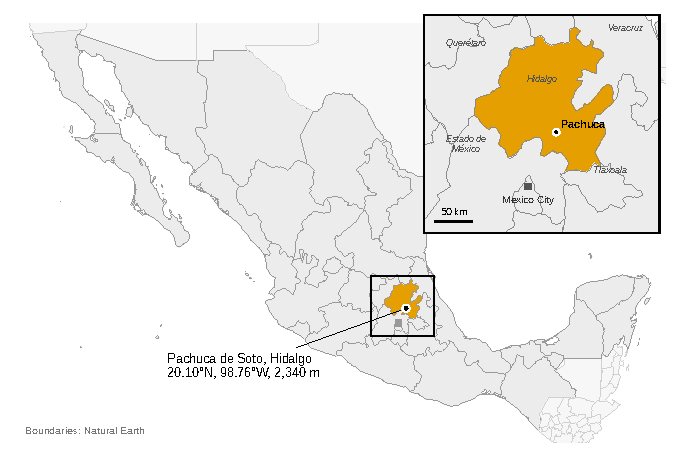
\includegraphics[width=0.62\linewidth]{figures/fig0_site.pdf}
\end{adjustwidth}
\caption{Location of the plant (Pachuca de Soto, Hidalgo). Boundaries: Natural Earth.}
\label{fig:site}
\end{figure}

\begin{figure}[H]
\begin{adjustwidth}{-\extralength}{0cm}
\centering
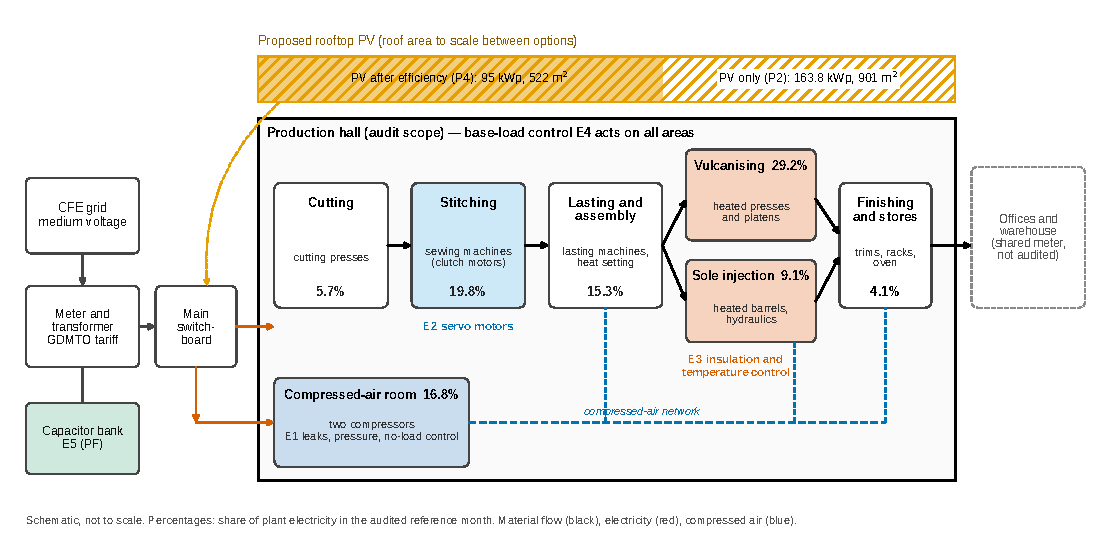
\includegraphics[width=\linewidth]{figures/fig_site_diagram.pdf}
\end{adjustwidth}
\caption{Plant layout and energy flows (schematic, not to scale). Percentages: share of plant electricity; E1--E5: measures.}
\label{fig:sitediagram}
\end{figure}

Table~\ref{tab:data} summarises the data and their status. Monthly electricity consumption, billed demand, power factor (PF) and the average price per kWh were transcribed from \nNMonths\ utility bills (January 2024--April 2026, Table~\ref{tab:billing}). Monthly production in pairs was taken from plant records for \nProdMonths\ of these months. During a walk-through audit in the first half of 2026 the audit team estimated the distribution of electricity use across twelve production areas for a reference month (April 2026). Significant energy uses were vulcanising (29.2\%), stitching (19.8\%), the compressed-air room (16.8\%) and sole injection moulding (9.1\%). Tariff charges for every month from January 2024 to October 2026 were retrieved from the utility~\cite{cfe2026gdmto} (Table~\ref{tab:tariffs}). The emission factor, fuel prices, grid mix and solar resource were taken from official or institutional sources (Table~\ref{tab:data}). Monetary values are in 2026 Mexican pesos (\MXN; kMXN and MMXN denote thousands and millions) excluding value-added tax (VAT), which firms recover. For reference, 1~USD = \nUSDRate~\MXN{}~\cite{cne2026ipgn}.

\begin{table}[H]
\centering
\caption{Data sources and their status.}
\label{tab:data}
\resizebox{\linewidth}{!}{%
\begin{tabular}{p{3.3cm}p{6.2cm}p{4.3cm}}
\toprule
Item & Content & Source / status \\
\midrule
Electricity bills & kWh, billed kW, PF and average price; Jan 2024--Apr 2026 (\nNMonths\ months) & Utility bills, transcribed (measured) \\
Production & Pairs per month; Apr 2024--Apr 2026 (\nProdMonths\ months) & Plant records (measured) \\
End-use split & Share of 12 areas in the reference month & Audit walk-through estimate \\
Tariff & GDMTO fixed, energy, distribution and capacity charges, Centro Oriente, monthly 2024--2026 &~\cite{cfe2026gdmto,dof2025tariffs} (official) \\
Billed-demand rule & $\min\{D_{\max},\,Q/(24\,d\,F_C)\}$, $F_C=0.55$; PF surcharge and bonus &~\cite{dof2025tariffs} (official) \\
Grid emission factor & 0.444 tCO$_2$e MWh$^{-1}$ (2024), still mandated for 2026 reporting &~\cite{semarnat2025fesen,semarnat2026aviso} (official) \\
Grid mix and gas imports & Gas-fired share of 2024 generation; US pipeline imports vs.\ consumption &~\cite{sener2025plan,eia2025mexico} \\
Fuel prices & Natural-gas wholesale index (12-month mean); LP-gas maximum price for Pachuca &~\cite{cne2026ipgn,profeco2026lpg} (official) \\
Solar resource & Monthly global and diffuse irradiation, 2001--2025 climatology &~\cite{nasapower} \\
Measure costs & Capital costs of PV, capacitor bank and compressed-air works & Audit quotations; other costs assumed (Table~\ref{tab:parameters}) \\
\bottomrule
\end{tabular}}
\end{table}

\subsection{Modelling and optimisation framework}
\label{sec:framework}
Figure~\ref{fig:framework} summarises the framework. Monthly simulation models of the energy baseline, the tariff, the demand-side measures and rooftop PV (Sections~\ref{sec:baseline}--\ref{sec:indicators}) evaluate any portfolio of options. Four optimisation problems are solved on top of these models. Let $G(\mathcal{E},k)$ denote annual grid purchases after implementing the set of measures $\mathcal{E}$ and a PV array of $k$~kWp, and $G_0$ the reference-year purchases.

\emph{Problem 1, right-sizing PV after efficiency.} For the full set of measures $\mathcal{E}^{\ast}$, find
\begin{equation}
k_4^{\ast} = \min\{k \ge 0 : G(\mathcal{E}^{\ast},k) \le G(\varnothing,k_2)\},
\label{eq:p4}
\end{equation}
where $k_2$ is the supply-only design. Because $G$ decreases monotonically in $k$, the problem is solved by bisection to 0.1~kWp.

\emph{Problem 2, efficiency-first pathways.} For each target reduction $\tau$ in grid purchases, measures are added in ascending order of CCE until $G \le (1-\tau)G_0$; if the target is not met, the smallest PV array that closes the gap is found by bisection. The supply-only pathway sizes PV directly from its specific yield for the same $\tau$. Power-factor correction is included in both pathways.

\emph{Problem 3, least-capital PV and storage design.} For a self-sufficiency target $\sigma$, find
\begin{equation}
\min_{k\in\mathcal{K},\,b\in\mathcal{B}} C(k,b) \quad \text{subject to} \quad S(k,b) \ge \sigma,
\label{eq:p3}
\end{equation}
where $C$ is capital cost, $S$ is hourly self-sufficiency simulated over 8,760 hours, $\mathcal{K}$ contains 19 PV sizes (0.6--2.4 times the annual net-zero size of each measure set, capped at 700~kWp) and $\mathcal{B}$ 25 battery sizes (0--2,400~kWh; Section~\ref{sec:nzmethod}). The 950 designs (two measure sets) are enumerated exhaustively, which guarantees the optimum on the grid without assumptions on the convexity of $S$, and each is valued under three compensation regimes. Monte Carlo simulation propagates parameter uncertainty through the monthly models for the designs obtained at central values.

\emph{Problem 4, joint cost-optimal design.} The fourth problem removes the sequencing assumption altogether. A linear programme built in the open energy-system optimisation model urbs (Section~\ref{sec:urbsmethod}) chooses simultaneously how much of each efficiency measure to adopt, the PV and battery capacities and the hourly operation of the plant's electricity system, with and without caps on grid emissions. Because it is solved independently of Problems 1--3, it tests whether efficiency first emerges from cost minimisation rather than being imposed, and it extends the analysis to deep decarbonisation, where storage becomes necessary.

\begin{figure}[H]
\begin{adjustwidth}{-\extralength}{0cm}
\centering
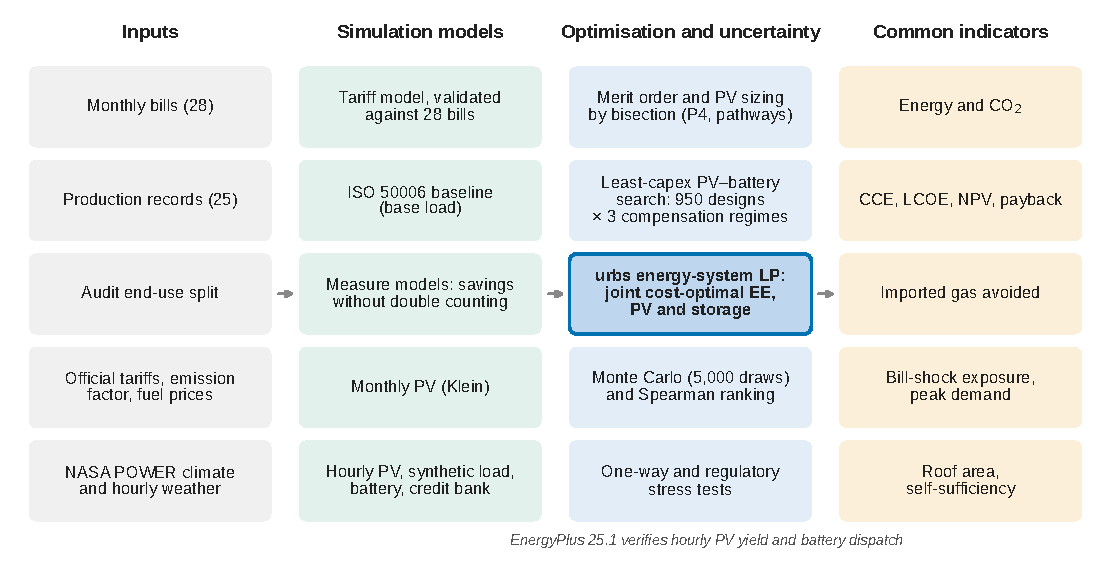
\includegraphics[width=0.92\linewidth]{figures/fig_framework.pdf}
\end{adjustwidth}
\caption{Modelling and optimisation framework.}
\label{fig:framework}
\end{figure}

\subsection{Energy baseline and performance indicator}
\label{sec:baseline}
Following ISO~50006~\cite{iso50006}, the energy baseline (EnB) relates monthly electricity use $E_m$ to production $P_m$ through ordinary least squares, $E_m = a + b\,P_m + \varepsilon_m$. The intercept $a$ is interpreted as production-independent (base) load. Three specifications were estimated and compared with the regression originally reported by the audit team: all \nNAll\ months; \nNExcl\ months excluding the documented 24-hour-shift months; and the original 16-month subset (April 2024--June 2025 plus September 2025). Model adequacy is reported through $R^2$ and the coefficient of variation of the root-mean-square error (CV-RMSE). The specification that excludes the 24-hour-shift months is used to define the base load targeted by the operational measure (E4).

\subsection{Tariff model and validation}
\label{sec:tariffmodel}
The GDMTO bill (pre-VAT) in month $m$ is
\begin{equation}
B_m = \big[c_f + c_e\,Q_m + (c_d + c_c)\,D^{b}_m\big]\,(1+\phi_m), \qquad D^{b}_m = \min\left\{D^{\max}_m,\ \frac{Q_m}{24\,d_m\,F_C}\right\},
\label{eq:bill}
\end{equation}
where $c_f$ is the fixed charge, $c_e$ the energy charge, $c_d$ and $c_c$ the distribution and capacity charges per kW, $Q_m$ the energy consumed, $d_m$ the days in the billing period and $F_C=0.55$ the load factor prescribed for GDMTO~\cite{dof2025tariffs}. Because GDMTO has no peak period, the capacity charge always applies the energy-based term; the distribution charge applies the smaller of measured maximum demand and the energy-based term~\cite{cfe2026gdmto}. The PF adjustment $\phi_m$ is a surcharge of $\tfrac{3}{5}(90/\mathrm{PF}-1)$ below 90\% PF and a bonus of $\tfrac{1}{4}(1-90/\mathrm{PF})$ at or above 90\%, capped at 120\% and 2.5\% respectively~\cite{dof2025tariffs}.

The model was validated by applying month-specific official charges to the recorded consumption, billed demand and PF of all \nNMonths\ months and comparing the result with the average price reported on each bill. The reported billed demand closely matches the energy-based term $Q_m/(24 d_m F_C)$ (mean ratio \nKWRatio). We therefore model billed demand with the energy-based term in all scenarios. Where $Q_m/(24 d_m F_C)$ falls below the measured peak, as appears to be the case here, a kWh saved reduces both the energy charge and the two demand charges. The avoided cost per kWh is then
\begin{equation}
v = c_e + \frac{c_d + c_c}{24\,\bar d\,F_C},
\label{eq:marginal}
\end{equation}
evaluated at the October 2026 charges and an average month length $\bar d = 30.4$ days. All scenarios use these charges with constant real prices. The reference year is May 2025--April 2026, the latest twelve billed months (\nRefMWh~MWh).

\subsection{Options appraised}
\paragraph{Demand-side measures}
Five measures derived from the audit were modelled (Table~\ref{tab:parameters}). They are applied sequentially to avoid double counting: E4 first scales all end uses, then component measures act on the remaining energy of their target areas.
\begin{itemize}
\item \textbf{E1 Compressed-air package}: leak detection and repair, reduction of discharge pressure and no-load control of the two compressors. The saving is 10--30\% of compressed-air energy (central 20\%)~\cite{doe2016compressed}. Capital cost follows the audit estimate, plus an annual ultrasonic leak survey.
\item \textbf{E2 Servo motors on sewing machines}: clutch motors in the stitching area are replaced with servo motors that save 50--75\% of motor energy (central 65\%)~\cite{nemesa2023}. Motors are assumed to use 50--85\% of stitching-area energy. The number of machines (\nNSewing\ in the central case) follows from the motor energy, a clutch-motor running power of 0.25--0.45~kW and the scheduled operating hours. It is multiplied by an installed unit cost.
\item \textbf{E3 Insulation of heated platens and barrels}: insulating jackets and improved temperature control on vulcanising presses and injection-unit barrels. The saving is 10--30\% of heater energy (central 20\%)~\cite{kent2018}. Heaters are assumed to account for 50--80\% of the energy of these areas.
\item \textbf{E4 Base-load (idle) control}: shutdown routines, timers and sub-metering that cut production-independent load by 5--20\% (central 10\%)~\cite{mouzon2007,kara2011}. The base load is taken as the EnB intercept.
\item \textbf{E5 Power-factor correction}: the 50~kVAr automatic capacitor bank proposed in the audit, raising PF to 0.95--0.99 (central 0.97). It saves money through the PF adjustment but not energy.
\end{itemize}

\paragraph{Supply-side options}
\textbf{S1 Rooftop PV} is the 163.8~kWp array (252 modules of 650~W) proposed in the audit, connected under the distributed-generation regime with monthly net metering. Monthly plane-of-array irradiation for a south-facing 20$^\circ$ tilt was computed from NASA POWER global and diffuse irradiation using the isotropic-sky monthly method of Klein~\cite{klein1977}. Generation applies a performance ratio of 0.75--0.85~\cite{reich2012} and 0.5\% per year degradation. Net metering reduces $Q_m$ and therefore the energy-based billed demand. A regulatory stress case removes this demand credit, so that PV offsets only the energy charge. Monthly surplus, if any, is conservatively assigned zero value.

\textbf{S2 Fuel substitution and electrification of heat} is assessed parametrically, per GJ of useful heat, because the plant's thermal fuel use was not metered during the audit. Five supply routes are compared: liquefied petroleum gas (LPG) or natural-gas boilers (efficiency 0.85), electric resistance, heat pumps (COP 2.5--4.0;~\cite{arpagaus2018,schlosser2020}) and recovery of compressor heat; more than 80\% of compressor input power becomes available heat~\cite{doe2016compressed}, and we conservatively assume that 50--80\% of input power (central 70\%) is recovered. Prices are the LPG maximum price for Pachuca in October 2026~\cite{profeco2026lpg} and the twelve-month mean of the national natural-gas wholesale index~\cite{cne2026ipgn}, doubled to approximate transport and distribution to an end user. Electricity is valued with Eq.~\eqref{eq:marginal}. Combustion emission factors follow~\cite{ipcc2006}. Because the plant's thermal fuel use is unknown, results are reported per GJ of useful heat and can be scaled by any annual fuel consumption.

\subsection{Common indicators}
\label{sec:indicators}
Each option and portfolio is evaluated with the same indicators:
\begin{itemize}
\item \emph{Energy}: annual grid purchases and the share avoided.
\item \emph{Emissions}: grid purchases multiplied by the official factor of 0.444~tCO$_2$e~MWh$^{-1}$, held constant because the official series rose over 2022--2024~\cite{cre2023fesen2022,cre2024fesen2023,semarnat2025fesen}. A decline of 3\% per year would lower lifetime avoided emissions by \nEFTrendDrop\% but would not change any monetary result.
\item \emph{Cost of conserved energy}: $\mathrm{CCE} = (I\cdot\mathrm{CRF}_{r,L} + C_{\mathrm{O\&M}})/\Delta E$~\cite{meier1982}, where $\mathrm{CRF}_{r,L}$ is the capital recovery factor at discount rate $r$ over life $L$. For PV the analogous metric is the levelised cost of electricity (LCOE). Both are compared with the avoided tariff $v$.
\item \emph{Economics}: NPV over 20 years at a 10\% real discount rate, with like-for-like reinvestment of short-lived measures, straight-line residual values and a PV inverter replacement in year 12; simple payback; and the net abatement cost, defined as the annualised negative NPV per tonne of CO$_2$.
\item \emph{Security and resilience}:
  \begin{itemize}
  \item imported natural gas avoided upstream, $\Delta E_{\mathrm{grid}}\cdot s_{\mathrm{gas}}\cdot h\cdot s_{\mathrm{imp}}$, with gas-fired share of generation $s_{\mathrm{gas}}=0.638$~\cite{sener2025plan}, heat rate $h=7.2$~GJ~MWh$^{-1}$ and import share $s_{\mathrm{imp}}=0.74$~\cite{eia2025mexico};
  \item exposure to an energy-price shock, measured as the increase in the annual bill if the energy charge rose by 50\%;
  \item the highest energy-implied billed demand, a proxy for proximity to the 100~kW threshold above which GDMTO customers must migrate to the time-of-use GDMTH tariff~\cite{cfe2026gdmto}; PV is not credited with peak reduction because cloudy days and evening operation make its contribution to the measured peak unreliable;
  \item the roof area required by PV;
  \item the sensitivity of value to a change in distributed-generation compensation.
  \end{itemize}
\end{itemize}

\subsection{Portfolios and efficiency-first pathways}
Four portfolios are compared with the baseline (P0): P1, the efficiency bundle (E1--E5); P2, supply only (the 163.8~kWp array); P3, both; and P4, efficiency first, in which the efficiency bundle is implemented and PV is then sized to reach the same grid purchases as P2. To generalise P4, we construct pathways for targets of 5--75\% reduction in grid purchases. The supply-only pathway sizes PV directly to the target (with PF correction in both pathways for fairness). The efficiency-first pathway adds measures in ascending order of CCE until the target is met and closes any remaining gap with PV.

\subsection{Uncertainty analysis}
Parameter uncertainty is propagated with \nMCN\ Monte Carlo draws from triangular distributions whose bounds are listed in Table~\ref{tab:parameters}. These cover measure savings and costs, PV cost, performance and degradation, discount rate (6--14\%) and real tariff escalation ($-1$ to $+2$\% per year). The grid-gas parameters do not affect monetary results; their ranges are reported for the imported-gas indicator as low and high bounds. We report 5th--95th percentiles, the probability that each portfolio has positive NPV, the probability that P4 outperforms P2 and Spearman rank correlations between inputs and the NPV difference P4$-$P2. One-way sensitivities are given in Appendix~\ref{app:sens}. The demand-credit rule for PV is treated as a discrete regulatory scenario rather than a random variable.

\subsection{Net-zero scenarios with renewables and storage}
\label{sec:nzmethod}
Two net-zero definitions are examined because they lead to different designs. \emph{Annual net-zero electricity} requires on-site PV generation to equal the plant's annual consumption, with the grid used as a seasonal buffer. Under the distributed-generation rules, net-metered surpluses are credited in kWh against later bills for up to 12 months, after which unused credits are paid at the local marginal price~\cite{cre2017dg}. We conservatively value expired credits at zero. \emph{Hourly self-sufficiency} measures the share of hourly consumption met on site by PV and a lithium-ion battery, a proxy for physical independence and resilience to supply interruptions. Targets of 70\%, 80\% and 90\% are analysed.

Because interval data are not available, an hourly load profile was synthesised for each reference-year month. It consists of an always-on load of 15~kW (range 8--25~kW, an assumption) and a flat load during scheduled operating hours that closes the monthly energy balance; during the three 24-hour-shift months production is spread over Monday--Saturday. Base-load control (E4) is assumed to reduce the always-on load first. Hourly PV output uses NASA POWER 2023 hourly global and diffuse irradiance at the site~\cite{nasapower}, transposed to the array plane with an isotropic-sky model and rescaled month by month to the 2001--2025 climatology, which gives a specific yield of \nSpecYieldHourly~kWh~kWp$^{-1}$, consistent with the monthly model. The battery follows a greedy self-consumption dispatch, with 85\% round-trip efficiency, a 15-year life and fixed O\&M of 2.5\% of capital per year~\cite{nrel2024atb}, 90\% usable depth of discharge, a power rating of 0.5~kW per kWh and an installed cost of 8,500~\MXN~kWh$^{-1}$ (an assumption anchored on the pack prices of about 200~USD~kWh$^{-1}$ reported in~\cite{nrel2024atb}; its influence is examined through a break-even analysis).

For each portfolio (supply only, or efficiency bundle first) we sweep PV capacity from 0.6 to 2.4 times the annual net-zero size, capped at the 0.7~MW distributed-generation limit~\cite{lse2025}, and battery capacity from 0 to 2,400~kWh, and retain the least-capital design that meets each self-sufficiency target. Each design is valued under three compensation regimes: monthly net metering with energy-based billed demand (the central case); net metering in which billed demand follows gross imports rather than net consumption; and net billing, in which imports are billed at the tariff and exports are paid 1.0~\MXN~kWh$^{-1}$. PV degradation of 0.5\% per year is applied to the PV share of the savings. Battery cost is explored through a break-even analysis; the other parameters of the net-zero module are held at their central values except the always-on load.

The five key designs were cross-validated in EnergyPlus 25.1~\cite{crawley2001}. An EPW file was built from the same rescaled NASA POWER hourly data, converted from the NASA POWER time stamps (UTC$-7$ at this longitude) to local clock time; PV was modelled with \texttt{Generator:\allowbreak{}PVWatts} (version 5, 14\% system losses, roof-mounted, 20$^\circ$ tilt, south) and a PVWatts inverter (DC/AC ratio 1.1, 96\% efficiency); storage with \texttt{ElectricLoadCenter:\allowbreak{}Storage:\allowbreak{}Simple} using the same capacity, power and efficiencies, AC-coupled and dispatched to track facility demand and store on-site surplus. The same hourly load was imposed through a schedule file, and EnergyPlus hourly purchased and surplus electricity were passed through the same net-metering bank and tariff.

\subsection{Joint cost-optimal design with urbs}
\label{sec:urbsmethod}
urbs is an open-source linear optimisation model for distributed energy systems developed at the Technical University of Munich~\cite{urbs}. It represents an energy system as commodities linked by processes and storage, and minimises the annualised cost of meeting an hourly demand. Here the plant is modelled as one site with one electricity bus over one year of 8,760 hours (Figure~\ref{fig:urbsstructure}). Grid purchases, rooftop PV, the battery and the four energy-saving measures supply the bus. The plant demand, exports and curtailment draw from it. The hourly load and PV output are those of Section~\ref{sec:nzmethod}.

\begin{figure}[H]
\begin{adjustwidth}{-\extralength}{0cm}
\centering
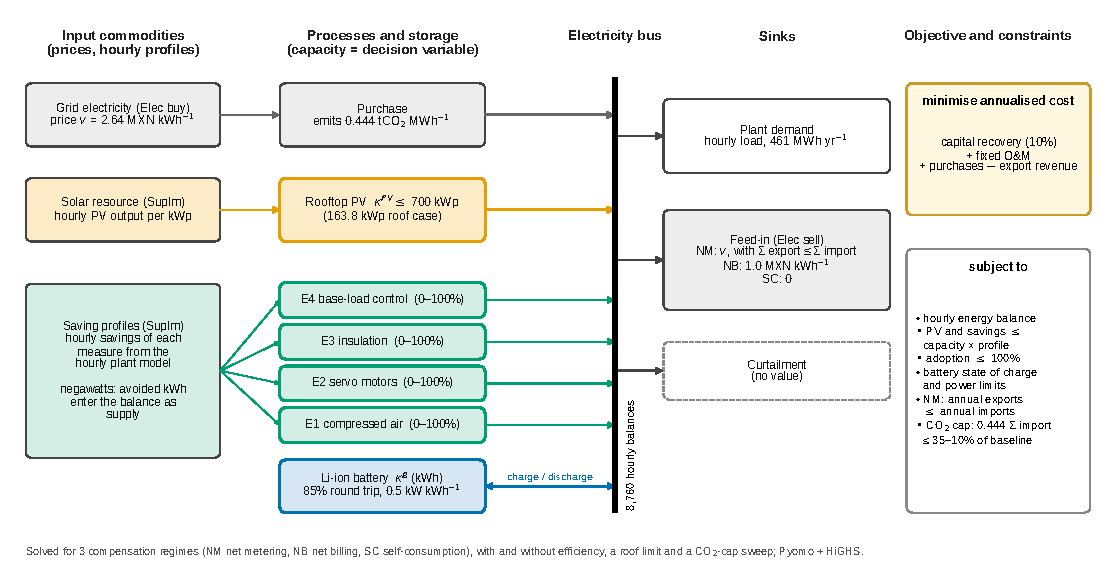
\includegraphics[width=\linewidth]{figures/fig_urbs_structure.pdf}
\end{adjustwidth}
\caption{Structure of the urbs model of the plant.}
\label{fig:urbsstructure}
\end{figure}

The efficiency measures enter as ``negawatt'' processes. Let $\hat{s}_{m,t}$ be the hourly saving of measure $m \in \mathcal{M}=\{\mathrm{E1},\ldots,\mathrm{E4}\}$ at full implementation, taken from the hourly model, and $a_m \in [0,1]$ the adopted fraction. The avoided kWh $a_m\hat{s}_{m,t}$ are supplied to the bus at the measure's investment cost, O\&M and lifetime, so that a measure competes with PV and storage as a resource, as the EE1st principle requires. With PV capacity $k$ (kWp) and hourly yield $y_t$ (kWh~kWp$^{-1}$), usable battery capacity $b$ (kWh), grid imports $g_t$, exports $x_t$, curtailment $c_t$, battery charge $q^{+}_t$, discharge $q^{-}_t$ and state of charge $e_t$, the programme is
\begin{align}
\min\quad & \sum_{m\in\mathcal{M}} a_m\left(\alpha_m I_m + F_m\right) + k\left(\alpha_{\mathrm{PV}} I_{\mathrm{PV}} + F_{\mathrm{PV}}\right) + b\left(\alpha_{\mathrm{B}} I_{\mathrm{B}} + F_{\mathrm{B}}\right) + \sum_{t=1}^{8760}\left(v\,g_t - p_x\,x_t\right) \label{eq:urbsobj}\\
\text{s.t.}\quad & g_t + k\,y_t + \sum_{m} a_m \hat{s}_{m,t} + q^{-}_t = d_t + x_t + c_t + q^{+}_t \qquad \forall t \label{eq:urbsbal}\\
& e_t = e_{t-1} + \eta\,q^{+}_t - q^{-}_t/\eta, \qquad 0 \le e_t \le b, \qquad q^{+}_t,\,q^{-}_t \le \rho\,b \qquad \forall t \label{eq:urbssto}\\
& 0 \le k \le \bar{k}, \qquad 0 \le a_m \le 1 \label{eq:urbscap}\\
& \textstyle\sum_t x_t \le \sum_t g_t \quad \text{(net metering only)} \label{eq:urbsnm}\\
& \varepsilon \textstyle\sum_t g_t \le \phi\,\varepsilon \sum_t d_t \quad \text{(emission cap)}, \label{eq:urbsco2}
\end{align}
where $d_t$ is the hourly demand without measures, $I$ and $F$ are investment and fixed O\&M costs, $\alpha$ is the capital recovery factor at the 10\% discount rate over each asset's lifetime, $\eta=\sqrt{0.85}$ is the one-way battery efficiency, $\rho$ the power-to-energy ratio (0.5~kW per kWh of nameplate capacity), $\varepsilon$ the grid emission factor and $\phi$ the cap as a fraction of baseline emissions. The battery starts and ends the year half full.

Grid purchases are priced at the marginal value $v$ of Equation~(\ref{eq:marginal}); this is appropriate because GDMTO demand charges are proportional to energy, whereas the fixed charges and the power-factor adjustment do not depend on the decisions optimised, which is also why power-factor correction (E5) is excluded. The PV investment cost includes the inverter replacement, and the array is limited to $\bar{k}=0.7$~MW, the distributed-generation limit. The savings of base-load control are assigned to the hours in which it reduces load, preserving its monthly energy. Three compensation regimes set the export price $p_x$: annual net metering, in which exports are credited at $v$ subject to Equation~(\ref{eq:urbsnm}); net billing, in which exports are paid 1.0~\MXN~kWh$^{-1}$; and self-consumption, in which exports have no value. Surplus PV output can be curtailed. Penalties of $10^{-3}$~\MXN~kWh$^{-1}$ on exports and battery throughput remove degenerate solutions with simultaneous import and export or simultaneous charge and discharge; they do not affect the results.

\begin{table}[H]
\caption{Scenarios solved with urbs.}
\label{tab:urbsruns}
\footnotesize
\begin{tabularx}{\linewidth}{p{3.2cm}Xr}
\toprule
Scenario set & Settings & Runs \\
\midrule
Compensation regimes & Net metering, net billing, self-consumption; no emission cap & 6 \\
Roof limit & Net metering; $\bar{k}=163.8$~kWp (audit layout) & 2 \\
Emission caps & Net metering; $\phi$ = 35, 30, 25, 20, 15, 10\% & 12 \\
Battery cost & Net metering; battery cost 75, 50, 25\% of central; no cap and $\phi$ = 20\% & 12 \\
\bottomrule
\end{tabularx}
\end{table}

Each scenario is solved twice, with the measures available ($a_m \in [0,1]$) and without them ($a_m = 0$, supply only), which isolates the contribution of efficiency at every point (Table~\ref{tab:urbsruns}). The \nUNRuns\ linear programmes, each with 8,760 hourly time steps, were solved with HiGHS through Pyomo in about \nUSolveMean~s each.

\subsection{Reproducibility, data and code}
\label{sec:repro}
The model is written in Python (NumPy, pandas, Matplotlib) and organised as a small package with scripts that regenerate every number, table and figure in this paper from the input data. All numbers quoted in the text are inserted automatically from the results files. The public repository contains the model code, the official tariff, price, emission-factor and climate series with their sources and access dates, all derived results files, the figures, the Monte Carlo seed and a README with run instructions. The urbs benchmark is generated by two further scripts (input preparation and solution) that run urbs (GPL-3.0, commit 37487e6) with Pyomo 6.8 and HiGHS in a separate Python environment specified in the repository. The plant's billing, production and end-use records are confidential and are not included; the repository documents their format so that the scripts can be run with them, or with another plant's data. Code is released under the MIT licence and public data, results and figures under CC~BY~4.0. The repository is archived on Zenodo (\url{https://doi.org/10.5281/zenodo.23419738}) and mirrored on GitHub (\url{https://github.com/kerdan85/efficiency-first-sme}).

To make the method usable beyond this plant, the same repository contains \texttt{ee1st}, a general-purpose implementation installable as a Python package from its \texttt{ee1st/} folder~\cite{ee1st2026}. A plant is described in a single case file that lists its bills, tariff, end-use split, candidate measures and PV and storage options; every numeric input can be given as a central value or as a (central, low, high) range with a data-status label (for example measured, official, literature, quote or assumption). From this file the toolkit produces the core indicators, portfolios, pathways, Monte Carlo statistics and net-zero designs described in Sections~\ref{sec:method}--\ref{sec:results}, together with a short report; the EnergyPlus cross-check is not part of it. Three tariff structures are supported: Q-based demand charges as in GDMTO, energy plus measured-peak demand charges as common in Europe and North America, and flat energy prices. Measures are declared as base-load, end-use or power-factor measures, and a production series is optional; without it the base load is supplied directly. The footwear case is included as a configuration file with its public inputs; when the confidential plant records are supplied, an automated test confirms that the toolkit reproduces the deterministic results of this paper exactly and the Monte Carlo statistics within sampling error. An explicitly synthetic example, which runs without any confidential data, shows the inputs for a plant under an energy-plus-demand tariff without production records.

%% ===================================================================
\section{Results}
\label{sec:results}

\subsection{Energy use, baseline and tariff}
Monthly consumption ranged from \nKWhMin\ to \nKWhMax~kWh (mean \nKWhMean~kWh), and billed demand reached \nKWMax~kW (Figure~\ref{fig:data}a). Power factor averaged \nPFMean\% and fell below the 90\% threshold in \nMonthsPFLow\ of \nNMonths\ months, incurring net PF adjustments of about \nPFSurcharge~k\MXN\ in the reference year at 2026 charges. Production explains only part of the variability (Figure~\ref{fig:data}b). Over all \nNAll\ months the regression gives $E = \nIntAll + \nSlopeAll\,P$ ($R^2 = \nRSqAll$, CV-RMSE \nCVAll\%). Excluding the 24-hour-shift months yields $E = \nIntExcl + \nSlopeExcl\,P$ ($R^2 = \nRSqExcl$, CV-RMSE \nCVExcl\%). The regression in the audit report ($E = \nIntOrig + \nSlopeOrig\,P$, $R^2 = \nRSqOrig$) is reproduced only with the non-contiguous 16-month subset and with one month transcribed as 34,200 instead of 32,400~kWh. With the corrected value the subset gives $R^2 = \nRSqOrigCorr$. Whatever the specification, the intercept is large: base load accounts for about \nBaseShare\% of the reference-year mean consumption. Much of the plant's electricity is therefore not proportional to output, a typical signature of idle equipment, compressed-air leakage and heaters kept at temperature~\cite{kara2011,gutowski2009}.

The tariff model reproduces the reported average price of each bill with a mean bias of \nTVBias\% and a mean absolute error of \nTVMape\% (maximum \nTVMax\%; Figure~\ref{fig:data}c). The small positive bias is consistent with minor charges not itemised in the transcribed data. Two consequences follow. First, the plant's billed demand is set by its monthly energy rather than its instantaneous peak. Under October 2026 charges, an avoided kWh is therefore worth $v = \nTMarg$~\MXN\ (\nTMargUSD~USD), of which only \nTEnergyShare\% is the energy charge itself. Second, billed demand exceeded 100~kW in \nMonthsKWHundred\ months, including three consecutive months during the 24-hour shifts. The load factors printed on the bills, if defined on measured maximum demand, imply measured peaks of \nDmaxImpMin--\nDmaxImpMax~kW, above the 100~kW GDMTO limit in \nMonthsDmaxImp\ of \nNMonths\ months. The plant therefore appears to qualify for reclassification to the time-of-use GDMTH tariff, a regulatory exposure discussed in Section~\ref{sec:discussion}. The reference-year bill is \nBillZero~M\MXN.

\begin{figure}[H]
\begin{adjustwidth}{-\extralength}{0cm}
\centering
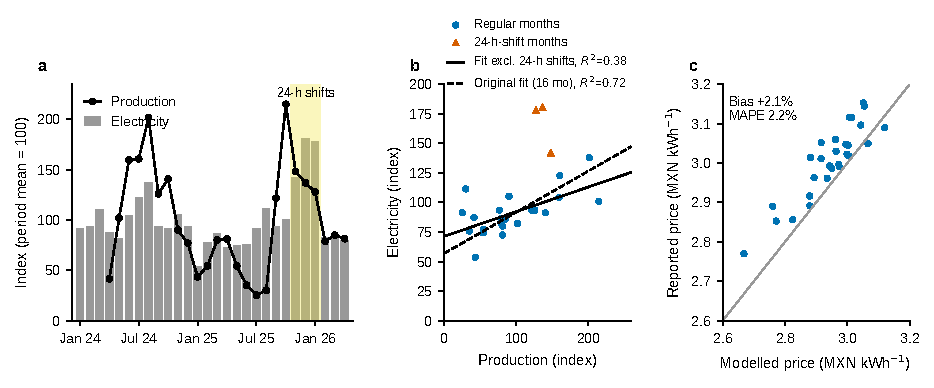
\includegraphics[width=\linewidth]{figures/fig1_data_baseline.pdf}
\end{adjustwidth}
\caption{Energy data, baseline and tariff validation: (a) monthly electricity and production (shading: 24-hour shifts); (b) baseline regressions; (c) reported versus modelled price.}
\label{fig:data}
\end{figure}

\subsection{Cost of conserved energy of demand-side measures}
\label{sec:cceresults}
Table~\ref{tab:measures} and Figure~\ref{fig:cce}b rank the measures. Base-load control (E4) is by far the cheapest resource, at \nCCEBase~\MXN~kWh$^{-1}$ for \nSavedBase~MWh per year. It is followed by insulation of heated platens and barrels (E3, \nCCEInsul), servo motors (E2, \nCCEServo, the largest single saving at \nSavedServo~MWh) and the compressed-air package (E1, \nCCECA). At central values all four lie well below the avoided tariff ($v = \nTMarg$) and also below the energy charge alone (\nTEnergy). Their 5th--95th percentile ranges, from \nCCELoBase--\nCCEHiBase\ for E4 to \nCCELoCA--\nCCEHiCA\ for E1, never reach the avoided tariff, and all measures remained below it simultaneously in \nProbAllBelow\% of Monte Carlo draws. Even if only the energy charge were avoided, E1 would still be below it in \nProbBelowEnergyCA\% of draws and the other measures in at least \nProbBelowEnergyServo\%. The measures are of the same order as the PV LCOE (\nPVLCOE~\MXN~kWh$^{-1}$, range \nLCOELo--\nLCOEHi). E4 was cheaper than PV in \nProbBelowPVBase\% of draws and E3 in \nProbBelowPVInsul\%, whereas E2 (\nProbBelowPVServo\%) and E1 (\nProbBelowPVCA\%) were usually slightly more expensive per kWh than PV. The distinctive value of the latter two lies less in their unit cost than in their small capital requirement and their contribution to lower demand (Section~\ref{sec:resil}). Power-factor correction saves no energy but removes the PF surcharge and earns the bonus, returning an NPV of \nNPVPFC~M\MXN\ on \nCapexPFC~k\MXN.

Individually, every measure has a payback of \nPBBase--\nPBPFC\ years (Table~\ref{tab:measures}). Combined (P1), they reduce grid purchases by \nEESavedMWh~MWh per year (\nEESavedPct\%), avoid \nCOOne~tCO$_2$ per year and require \nCapexOne~M\MXN\ (\nCapexOneUSD~kUSD) for an NPV of \nNPVOne~M\MXN.

\begin{table}[H]
\centering
\caption{Stand-alone appraisal of each option (CCE: for PV, LCOE; 5th--95th percentiles in brackets).}
\label{tab:measures}
\resizebox{\linewidth}{!}{%
\begin{tabular}{lrrlrrrr}
\toprule
Option & Capex & Electricity saved & CCE / LCOE & Bill saving, yr 1 & NPV & Payback & CO$_2$ avoided \\
 & (kMXN) & (MWh yr$^{-1}$) & (MXN kWh$^{-1}$) & (kMXN yr$^{-1}$) & (MMXN) & (yr) & (t yr$^{-1}$) \\
\midrule
E4 Base-load (idle) control & 40 & 30.4 & 0.21 [0.11--0.37] & 82 & 0.64 & 0.5 & 13.5 \\
E3 Insulation of heated platens/barrels & 100 & 23.0 & 0.82 [0.53--1.41] & 61 & 0.36 & 1.6 & 10.2 \\
E2 Servo motors on sewing machines & 241 & 41.5 & 0.94 [0.73--1.47] & 111 & 0.61 & 2.2 & 18.4 \\
E1 Compressed-air package & 50 & 15.5 & 1.04 [0.78--1.74] & 41 & 0.21 & 1.5 & 6.9 \\
E5 Power-factor correction (50 kVAr) & 85 & 0.0 & -- & 36 & 0.21 & 2.4 & 0.0 \\
S1 Rooftop PV (163.8 kWp) & 1{,}802 & 250.0 & 0.92 [0.74--1.20] & 670 & 3.57 & 2.8 & 111.0 \\
\bottomrule
\end{tabular}}
\end{table}


\begin{figure}[H]
\begin{adjustwidth}{-\extralength}{0cm}
\centering
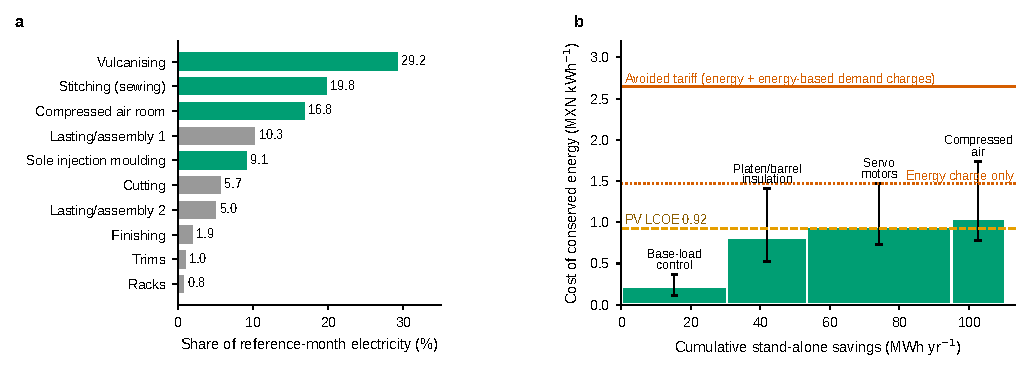
\includegraphics[width=\linewidth]{figures/fig2_enduses_cce.pdf}
\end{adjustwidth}
\caption{End uses and conservation supply curve: (a) electricity share by area; (b) CCE of each measure (whiskers: 5th--95th percentiles).}
\label{fig:cce}
\end{figure}

\subsection{Portfolio comparison}
Table~\ref{tab:portfolios} and Figure~\ref{fig:portfolios} compare the portfolios. Supply-only PV (P2) generates \nPVGen~MWh per year with a specific yield of \nSpecYield~kWh~kWp$^{-1}$. It cuts grid purchases by \nGridTwo\% and has a larger absolute NPV (\nNPVTwo~M\MXN) than the efficiency bundle (\nNPVOne~M\MXN), because it is a larger investment. Per peso invested, however, efficiency returns more: NPV/capex is \nNPVCapBase\ for E4 and between \nNPVCapMinEE\ and \nNPVCapMaxEE\ for E1--E3, against \nNPVCapPV\ for PV, and P1 beats P2 on this ratio in \nProbNPVCapex\% of Monte Carlo draws.

The efficiency-first portfolio (P4) reaches the same grid purchases as P2 (\nGridMWhFour~MWh per year, within \nGridDiffFour~MWh) with \nKWpFour~kWp of PV instead of 163.8~kWp. It requires \nCapexSaveFour\% less capital (\nCapexFour\ versus \nCapexTwo~M\MXN) and \nRoofSaveFour\% less roof (\nRoofFour\ versus \nRoofTwo~m$^2$), and achieves a higher NPV (\nNPVFour~M\MXN, $+\nNPVGainFour$~M\MXN). Emissions fall by \nCOFour~t per year in both cases (\nCOPctFour\% of the baseline \nCOBase~t). P4 also lowers the energy-implied peak from \nPeakTwo\ to \nPeakFour~kW, which PV alone cannot do. Installing the efficiency bundle together with the full 163.8~kWp array (P3) cuts grid purchases by \nGridThree\% and emissions by \nCOThree~t per year, with the largest NPV (\nNPVThree~M\MXN) but also the largest capital requirement (\nCapexThree~M\MXN). Net abatement costs are negative for every portfolio, between \nCostTOne\ and \nCostTTwo~\MXN~tCO$_2^{-1}$.

\begin{table}[H]
\centering
\caption{Portfolio comparison on common indicators.}
\label{tab:portfolios}
\resizebox{\linewidth}{!}{%
\begin{tabular}{lrrrrrrrrr}
\toprule
Portfolio & Capex & NPV & Grid purchases & Reduction & Residual CO$_2$ & Peak demand & Shock exposure & Imported gas & PV roof \\
 & (MMXN) & (MMXN) & (MWh yr$^{-1}$) & (\%) & (t yr$^{-1}$) & (kW) & (kMXN yr$^{-1}$) & (GJ yr$^{-1}$) & (m$^2$) \\
\midrule
P0 Baseline & 0.00 & 0.00 & 461 & 0 & 205 & 157 & 342 & 0 & 0 \\
P1 Efficiency bundle (E1--E5) & 0.52 & 1.84 & 356 & 23 & 158 & 124 & 257 & 357 & 0 \\
P2 Supply only: PV 163.8 kWp & 1.80 & 3.57 & 211 & 54 & 94 & 157 & 156 & 850 & 901 \\
P3 Efficiency bundle + PV 163.8 kWp & 2.32 & 5.11 & 111 & 76 & 49 & 124 & 80 & 1{,}188 & 901 \\
P4 Efficiency first + PV 94.9 kWp & 1.56 & 3.80 & 211 & 54 & 94 & 124 & 152 & 850 & 522 \\
\bottomrule
\end{tabular}}
\end{table}


\begin{figure}[H]
\begin{adjustwidth}{-\extralength}{0cm}
\centering
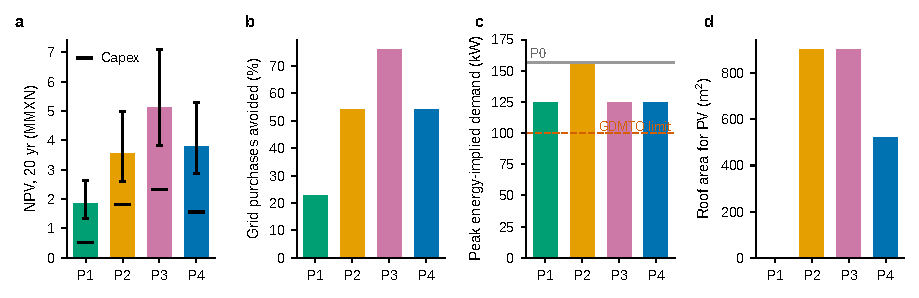
\includegraphics[width=\linewidth]{figures/fig3_portfolios.pdf}
\end{adjustwidth}
\caption{Portfolio indicators: (a) NPV and capital cost; (b) cut in grid purchases; (c) peak billed demand; (d) PV roof area.}
\label{fig:portfolios}
\end{figure}

\subsection{Efficiency-first pathways}
Figure~\ref{fig:pathways} generalises the comparison across reduction targets. Up to the \nEESavedPct\% reduction delivered by the efficiency bundle, efficiency measures alone meet the target and no PV is needed. Beyond that point PV is still required, but the array is always smaller than in the supply-only pathway. At a 50\% target, for instance, the efficiency-first pathway needs \nPathEKWp~kWp instead of \nPathSKWp~kWp, \nPathECapex\ instead of \nPathSCapex~M\MXN\ of capital (\nPathCapexSave\% less) and \nPathERoof\ instead of \nPathSRoof~m$^2$ of roof, with an NPV gain of \nPathNPVGain~M\MXN. The NPV gain is positive for every target. It is largest where efficiency alone meets the target and remains roughly constant at intermediate targets, where both pathways add PV at the same marginal value. It rises again above about 65\%, where the supply-only array starts to produce monthly surpluses that net metering does not remunerate in this model. The steps at low targets arise because measures are added as discrete units in merit order and can exceed the target.

\begin{figure}[H]
\begin{adjustwidth}{-\extralength}{0cm}
\centering
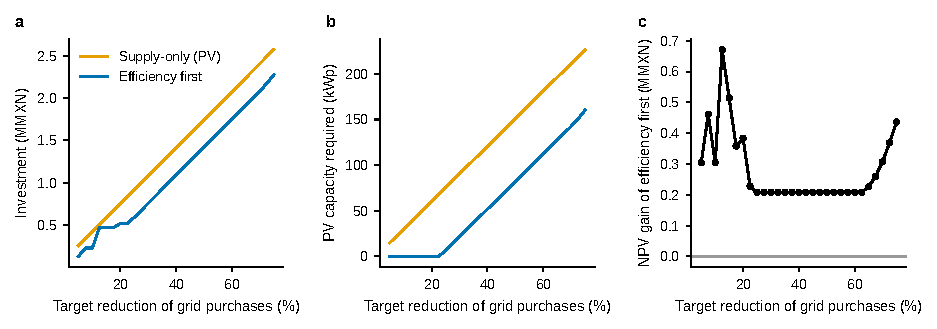
\includegraphics[width=\linewidth]{figures/fig4_pathways.pdf}
\end{adjustwidth}
\caption{Supply-only versus efficiency-first pathways: (a) capital; (b) PV capacity; (c) NPV gain of efficiency first.}
\label{fig:pathways}
\end{figure}

\subsection{Energy security and resilience}
\label{sec:resil}
The security indicators favour efficiency in ways that the averaged economics do not reveal (Figure~\ref{fig:resilience}).
\begin{itemize}
\item \emph{Regulatory stress.} If distributed-generation output no longer reduced billed demand, for example under a move from net metering to net billing, the NPV of the PV array would fall by \nPVStressDrop\% to \nNPVPVStress~M\MXN. The NPV of the efficiency bundle would be unchanged (\nNPVEEStress~M\MXN), because its savings reduce consumption behind the meter.
\item \emph{Energy-price shock.} A 50\% increase in the energy charge would raise the baseline bill by \nShockZero~k\MXN\ per year. The efficiency bundle cuts this exposure by \nShockCutOne\%, and P4 cuts it by \nShockCutFour\%, at least as much as P2 but with less capital.
\item \emph{Imported gas.} Upstream, the grid electricity avoided by P1 corresponds to about \nGasOne~GJ per year of imported natural gas (\nGasOneLo--\nGasOneHi~GJ across the parameter ranges), and that avoided by P2 and P4 to \nGasTwo~GJ (\nGasTwoLo--\nGasTwoHi~GJ).
\item \emph{Tariff-class threshold.} Efficiency reduces the highest energy-implied billed demand by \nPeakCutOne~kW. Neither this indicator in the surge months nor the measured peaks implied by the bills fall below the 100~kW GDMTO limit, so peak management (scheduling of compressors, presses and heaters) would be needed if the plant is reclassified.
\end{itemize}

\begin{figure}[H]
\begin{adjustwidth}{-\extralength}{0cm}
\centering
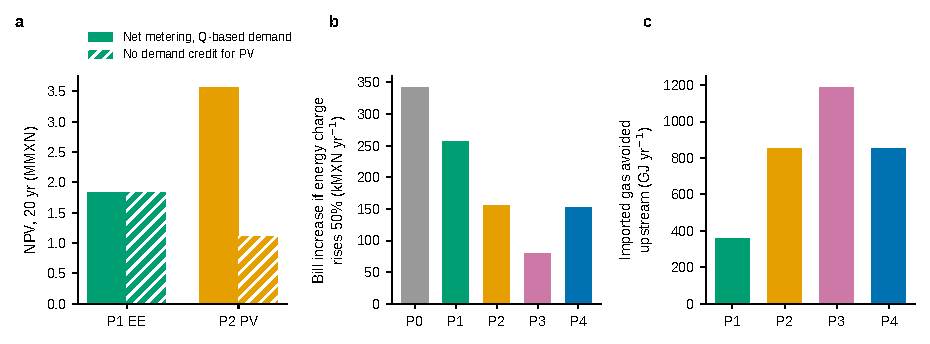
\includegraphics[width=\linewidth]{figures/fig5_resilience.pdf}
\end{adjustwidth}
\caption{Resilience indicators: (a) NPV with and without PV demand credit; (b) bill increase if the energy charge rises 50\%; (c) imported gas avoided.}
\label{fig:resilience}
\end{figure}

\subsection{Fuel substitution and electrification of heat}
\label{sec:thermal}
Per GJ of useful heat, an LPG boiler costs \nHeatLPG~\MXN\ and emits \nCOLPG~kgCO$_2$. A natural-gas boiler costs \nHeatNG~\MXN\ and emits \nCONG~kgCO$_2$ (Figure~\ref{fig:thermal}). Electric resistance heating at the avoided tariff costs \nHeatRes~\MXN~GJ$^{-1}$ and emits \nCORes~kgCO$_2$~GJ$^{-1}$, more than either fuel on both counts. A heat pump with COP~3 costs \nHeatHPThree~\MXN\ and emits \nCOHPThree~kgCO$_2$ per GJ. It beats LPG on cost for any COP above \nCOPBELPG\ and on emissions above \nCOPCOLPG. Against pipeline natural gas, however, a heat pump breaks even on emissions at COP \nCOPCONG\ but on cost only at COP \nCOPBENG, because wholesale gas is cheap relative to GDMTO electricity. Electrification is therefore a strong option where the plant burns LPG and a weak one where pipeline gas is available, unless electricity prices or gas prices change.

Efficiency interacts with electrification in two ways. First, it creates headroom: the \nEESavedMWh~MWh saved each year by P1 could supply about \nHeadroomGJ~GJ of useful heat through a COP-3 heat pump without increasing grid purchases above the baseline. Second, it reduces the heat available for recovery. Compressor heat that could be recovered falls from about \nCAHeatBefore\ to \nCAHeatAfter~GJ per year once E1 and E4 are implemented. Recovery projects should therefore be sized after the compressed-air system has been optimised, not before.

\begin{figure}[H]
\begin{adjustwidth}{-\extralength}{0cm}
\centering
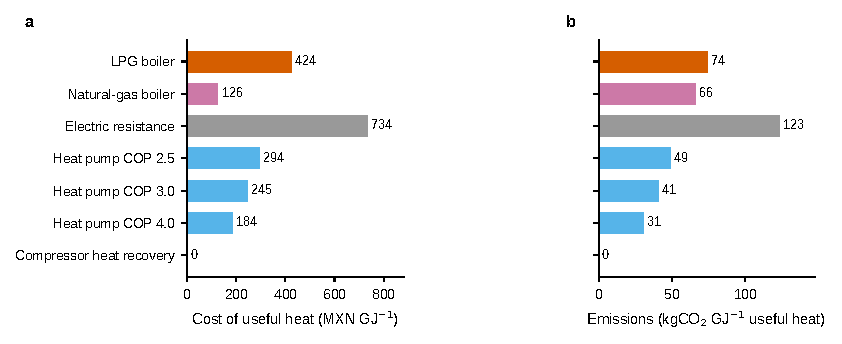
\includegraphics[width=\columnwidth]{figures/fig6_thermal.pdf}
\end{adjustwidth}
\caption{Heat supply routes: (a) cost and (b) emissions per GJ of useful heat.}
\label{fig:thermal}
\end{figure}

\subsection{Uncertainty}
All portfolios had positive NPV in every Monte Carlo draw (Figure~\ref{fig:uncertainty}a). The 5th--95th percentile ranges were \nMCLoOne--\nMCHiOne~M\MXN\ for P1, \nMCLoTwo--\nMCHiTwo\ for P2 and \nMCLoFour--\nMCHiFour\ for P4. P4 outperformed P2 in \nProbFourTwo\% of draws. The advantage of efficiency first is driven mainly by the achievable base-load saving ($\rho = \nRhoBase$), followed by the insulation saving ($\rho = \nRhoInsul$) and, at similar magnitude, the servo saving ($\rho = \nRhoServo$) and PV cost ($\rho = \nRhoPVCost$). It shrinks when PV performs better than expected ($\rho = \nRhoPR$; Figure~\ref{fig:uncertainty}b). One-way sensitivities (Appendix~\ref{app:sens}) confirm that no single parameter within its range reverses the sign of any portfolio NPV.

\begin{figure}[H]
\begin{adjustwidth}{-\extralength}{0cm}
\centering
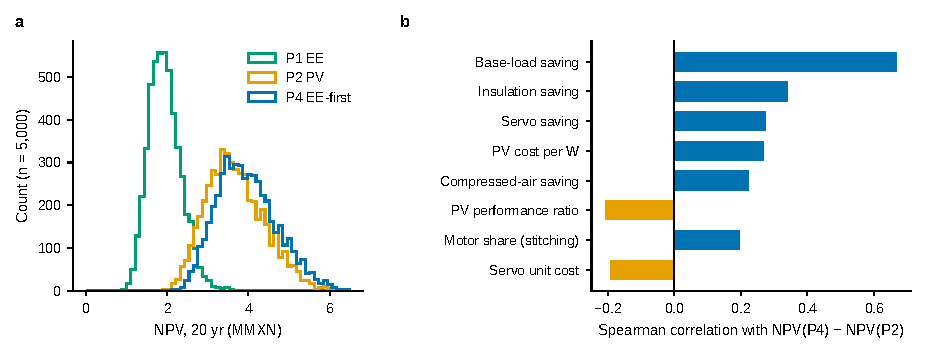
\includegraphics[width=\linewidth]{figures/fig7_uncertainty.pdf}
\end{adjustwidth}
\caption{Uncertainty (\nMCN\ draws): (a) NPV distributions; (b) main drivers of the NPV difference P4 $-$ P2.}
\label{fig:uncertainty}
\end{figure}

\subsection{Pathways to net-zero electricity}
\label{sec:nzresults}
Annual net-zero electricity is technically and economically within reach (Figure~\ref{fig:netzero}). Without efficiency, the plant needs \nKWpNZS~kWp of PV on \nRoofNZS~m$^2$ of roof (\nCapexNZS~M\MXN). With the efficiency bundle first it needs \nKWpNZE~kWp on \nRoofNZE~m$^2$ (\nCapexNZE~M\MXN, including the measures), that is \nNZKWpSave~kWp and \nNZRoofSave~m$^2$ less, and its NPV is higher (\nNPVNZE\ versus \nNPVNZS~M\MXN). Under net metering with a 12-month credit bank the annual bill falls to the fixed charge of about \nNZResidualBill~k\MXN, and no credits expire, because the seasonal surplus of the dry months is used during the high-consumption winter months (Figure~\ref{fig:netzero}c). Both designs stay well below the 0.7~MW distributed-generation limit. Roof space is the binding physical constraint. The usable roof area is not documented; the audit's 252-module layout implies at least about \nRoofTwo~m$^2$. On that area the full efficiency bundle plus the 163.8~kWp array (P3) cuts grid purchases by \nGridThree\%, against \nGridTwo\% for the array alone, whereas annual net zero would need about \nNZRoofSave~m$^2$ more roof without efficiency than with it. The less roof a plant has, the more efficiency first determines how close it can get to net zero.

Annual net zero is not physical independence. Without storage only \nSSNZE\% of hourly consumption is met on site, and gross grid imports remain \nImpNZE~MWh per year in the efficiency-first design (\nCOGrossNZE~tCO$_2$ on a location basis) and \nImpNZS~MWh in the supply-only design. Above about \nFirstBattery\% self-sufficiency storage is needed, from about \nFirstOversizeE--\nFirstOversizeS\% the least-cost designs also oversize the array, and the cost rises steeply (Figure~\ref{fig:netzero}a). The least-capital efficiency-first design for 80\% self-sufficiency combines \nKWpSSE~kWp with \nBatSSE~kWh (\nCapexSSE~M\MXN, NPV \nNPVSSE~M\MXN); the supply-only equivalent needs \nKWpSSS~kWp and \nBatSSS~kWh, \nSSEightyCapexSave~M\MXN\ more, and has an NPV of only \nNPVSSS~M\MXN, which turns negative if billed demand follows gross imports (\nNPVImpSSS~M\MXN). At 90\% the efficiency-first design needs \nKWpSSNE~kWp and \nBatSSNE~kWh (\nCapexSSNE~M\MXN) and its NPV turns negative (\nNPVSSNE~M\MXN). The highest self-sufficiency within the range explored (PV up to 2.4 times the annual net-zero array or 0.7~MW, and up to 2,400~kWh of storage) is about \nMaxSSE\%, with \nMaxSSKWp~kWp and \nMaxSSBat~kWh. Efficiency first lowers the capital required at every self-sufficiency level. The advantage comes mainly from lower total consumption, which shrinks the array: a supply-only design given the lower night load of the efficiency-first plant still needs \nSupplyLowNightCapex~M\MXN\ for 80\% self-sufficiency.

Storage does not pay under the current rules. Under net metering the grid already acts as a free, lossless seasonal store, so adding 200~kWh to the efficiency-first net-zero design raises self-sufficiency by \nBatMargSS\ percentage points but changes NPV by \nBatMargNM~M\MXN. The loss shrinks if billed demand follows gross imports (\nBatMargImp~M\MXN) or under net billing (\nBatMargNB~M\MXN), but remains negative at current battery costs (Figure~\ref{fig:netzero}b). Storage would break even only with battery costs \nBatBENB\% lower under net billing or \nBatBEImp\% lower under import-based demand charges, and never under net metering, where round-trip losses add to net imports. The value of storage for this plant is therefore resilience: the 80\% design holds about \nAutoSSE~hours of the always-on load. These results depend on the synthetic profile. Self-sufficiency of the annual net-zero designs ranges from \nNightSSLo\% to \nNightSSHi\% across the assumed always-on loads.

The EnergyPlus runs verify the PV yield and the battery dispatch of the Python model; they use the same synthetic load, weather, credit bank and tariff, so they do not test those inputs (Table~\ref{tab:energyplus}). For the designs with storage, self-sufficiency differs by at most \nEPSSDiffBat\ percentage points and grid imports by at most \nEPImpDiffBat\%; for the annual net-zero designs without storage the difference is at most \nEPSSDiffNZ\ points. EnergyPlus DC output is within \nEPDCvsPy\% of the Python AC output, and its AC yield (\nEPYield~kWh~kWp$^{-1}$) is \nEPYieldDiff\% lower mainly because the PVWatts inverter efficiency (96\%) is applied on top of 14\% system losses, whereas the Python model uses a single performance ratio of 0.80. Sized with the EnergyPlus yield, annual net zero requires \nEPKWpNZE~kWp with efficiency first and \nEPKWpNZS~kWp without it (a gap of \nEPKWpSave~kWp), and the NPVs become \nEPNPVNZE\ and \nEPNPVNZS~M\MXN, so the ranking is unchanged.

\begin{table}[H]
\centering
\caption{Net-zero designs: Python model versus EnergyPlus 25.1 (annual values).}
\label{tab:energyplus}
\resizebox{\linewidth}{!}{%
\begin{tabular}{lrrrrrr}
\toprule
Design & PV (kWp) & Battery (kWh) & PV output (MWh) & Grid imports (MWh) & Exports (MWh) & Self-sufficiency (\%) \\
\midrule
NZ-S annual net zero, supply only & 302.7 & 0 & 461 / 441 & 199 / 200 & 199 / 180 & 56.8 / 56.6 \\
NZ-E annual net zero, efficiency first & 233.6 & 0 & 356 / 340 & 152 / 153 & 152 / 137 & 57.3 / 57.1 \\
80\% self-sufficiency, supply only & 423.7 & 400 & 645 / 617 & 91 / 89 & 260 / 229 & 80.3 / 80.7 \\
80\% self-sufficiency, efficiency first & 350.4 & 300 & 534 / 510 & 71 / 70 & 238 / 213 & 80.0 / 80.4 \\
90\% self-sufficiency, efficiency first & 467.2 & 800 & 711 / 680 & 35 / 33 & 374 / 341 & 90.2 / 90.7 \\
NZ-S re-sized with EnergyPlus yield & 316.5 & 0 & -- / 461 & -- / 197 & -- / 197 & -- / 57.2 \\
NZ-E re-sized with EnergyPlus yield & 244.3 & 0 & -- / 356 & -- / 150 & -- / 150 & -- / 57.7 \\
\bottomrule
\end{tabular}}
\end{table}


\begin{figure}[H]
\begin{adjustwidth}{-\extralength}{0cm}
\centering
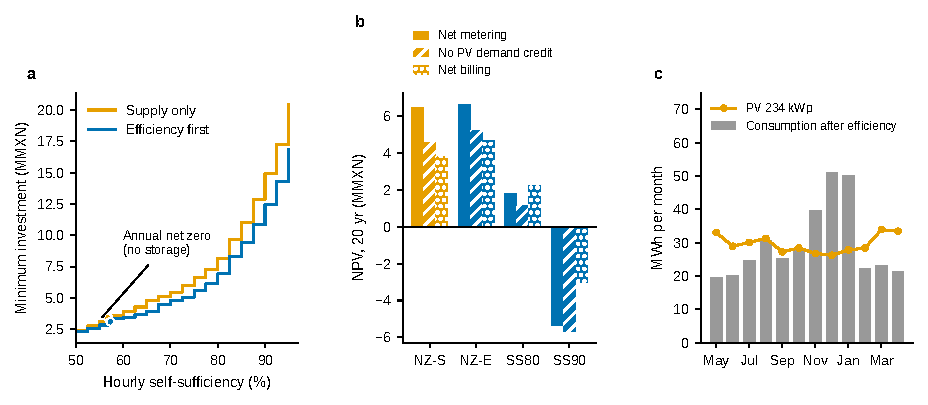
\includegraphics[width=\linewidth]{figures/fig8_netzero.pdf}
\end{adjustwidth}
\caption{Net zero with PV and storage: (a) least capital by self-sufficiency target; (b) NPV under three compensation regimes; (c) monthly balance of the efficiency-first net-zero design.}
\label{fig:netzero}
\end{figure}

%% ===================================================================
\subsection{Joint cost-optimal design with urbs}
\label{sec:urbsresults}

\subsubsection{Cost-optimal designs under three compensation regimes}
Without an emission cap and under annual net metering, the cost-optimal supply-only design is a \nUPVNMS~kWp array without storage (Table~\ref{tab:urbs}). This is the annual net-zero size found by the hourly design search in Section~\ref{sec:nzresults}, with the same hourly self-sufficiency of \nUSSNMS\%, so the two models describe the same system. When efficiency is available, the optimiser adopts base-load control and insulation in full but not the servo motors or the compressed-air package. It installs \nUPVNME~kWp of PV and lowers the annualised cost from \nUCostNMS\ to \nUCostNME~k\MXN\ (\nUCostNMSave\%). This choice follows the merit order of Section~\ref{sec:cceresults}. Under annual net metering every kWh of PV output is worth the full tariff, so a measure enters only if its CCE is below the PV LCOE, and E2 and E1 lie just above it.

As soon as PV output loses part of its value, all four measures enter the optimum. With PV limited to the 163.8~kWp array, without export compensation, or with net billing at 1.0~\MXN~kWh$^{-1}$, efficiency lowers the annualised cost by \nUCostRLSave\%, \nUCostSCSave\% and \nUCostNBSave\%, respectively. Under net billing the export price exceeds the PV LCOE, so the array grows to the 0.7~MW limit with or without efficiency. In no regime are batteries part of the cost-optimal design without an emission cap.

\begin{table}[H]
\caption{Cost-optimal designs from urbs without an emission cap (grid only: 1{,}218~kMXN~yr$^{-1}$).}
\label{tab:urbs}
\footnotesize
\resizebox{\linewidth}{!}{%
\begin{tabular}{llrrrrrr}
\toprule
Compensation regime & Efficiency & Measures adopted & PV (kWp) & Battery (usable kWh) & Grid imports (MWh) & CO$_2$ (t) & Cost (kMXN yr$^{-1}$) \\
\midrule
Net metering & with & E3, E4 & 269 & 0 & 172 & 76 & 391 \\
 & without & -- & 303 & 0 & 199 & 88 & 412 \\
\midrule
Net billing (1.0 MXN kWh$^{-1}$) & with & E1--E4 & 700 & 0 & 118 & 53 & 518 \\
 & without & -- & 700 & 0 & 162 & 72 & 615 \\
\midrule
Self-consumption only & with & E1--E4 & 164 & 0 & 177 & 79 & 772 \\
 & without & -- & 208 & 0 & 232 & 103 & 897 \\
\midrule
Net metering, PV $\le$ 163.8 kWp & with & E1--E4 & 164 & 0 & 177 & 79 & 585 \\
 & without & -- & 164 & 0 & 261 & 116 & 782 \\
\bottomrule
\end{tabular}}
\end{table}


\subsubsection{Decarbonisation frontier and order of adoption}
Caps on gross grid emissions trace the cost-optimal decarbonisation frontier (Figure~\ref{fig:urbs}). The unconstrained optima already reduce gross grid CO$_2$ to \nUCOONME\% of the baseline with efficiency and \nUCOONMS\% without it. As the cap tightens, the optimiser adopts resources in a clear order (Figure~\ref{fig:urbs}c). It first completes the efficiency bundle: at a 35\% cap the servo motors are adopted at \nUEtwoAdoptThirtyFive\%, and all measures are adopted from 30\% onwards. It then expands PV and finally adds storage. Batteries enter at a cap of \nUFirstBatS\% without efficiency but only at \nUFirstBatE\% with it. At a 20\% cap the efficiency-first optimum needs \nUPVTwentyE~kWp of PV and \nUBatTwentyE~kWh of storage instead of \nUPVTwentyS~kWp and \nUBatTwentyS~kWh. At 10\% it needs \nUPVTenE~kWp and \nUBatTenE~kWh instead of \nUPVTenS~kWp and \nUBatTenS~kWh.

The cost of the frontier rises steeply once storage is required (Figure~\ref{fig:urbs}a). With efficiency, the annualised cost is \nUCostThirtyE~k\MXN\ at a 30\% cap and \nUCostTwentyE~k\MXN\ at 20\%, against \nUCostThirtyS\ and \nUCostTwentyS~k\MXN\ without it. Across the caps examined, efficiency lowers the annualised cost of meeting the cap by \nUCapSaveMin--\nUCapSaveMax\%. At a 10\% cap the annualised cost is \nUCostTenE~M\MXN\ with efficiency and \nUCostTenS~M\MXN\ without, both above the \nUGridCost~k\MXN\ per year of buying all electricity from the grid. Net grid purchases are close to zero along the frontier, because annual exports offset imports under net metering. Storage then accounts for \nUBatShareTenE\% of the annualised cost with efficiency and \nUBatShareTenS\% without it, whereas the measures account for only \nUEEShareTenE\% (Figure~\ref{fig:urbs}d).

\begin{figure}[H]
\begin{adjustwidth}{-\extralength}{0cm}
\centering
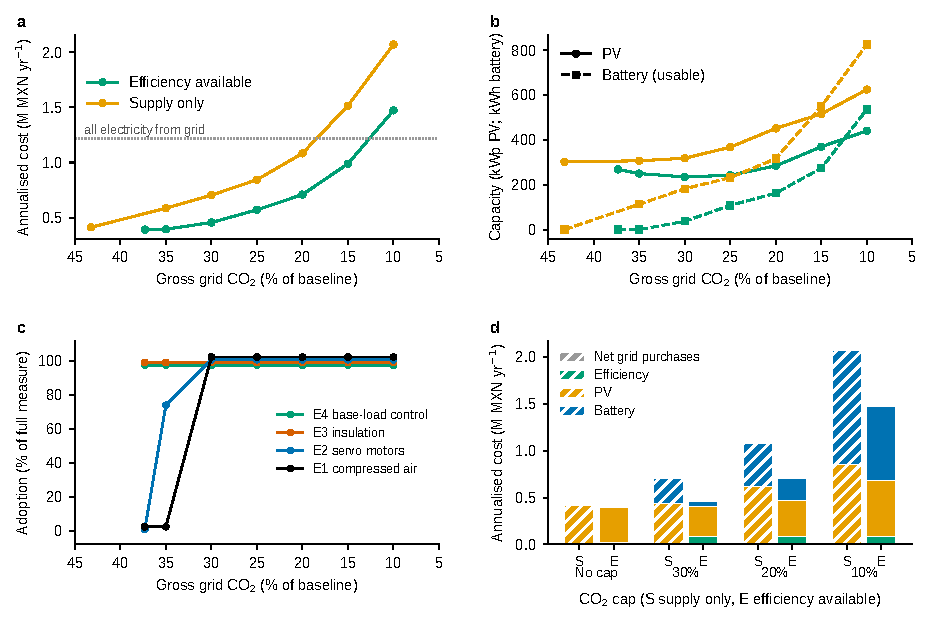
\includegraphics[width=\linewidth]{figures/fig9_urbs.pdf}
\end{adjustwidth}
\caption{Cost-optimal decarbonisation frontier from urbs (net metering): (a) annualised cost; (b) PV and battery capacity; (c) adoption of each measure; (d) annualised cost by component.}
\label{fig:urbs}
\end{figure}

\subsubsection{Hourly operation}
Figure~\ref{fig:urbsdispatch} shows how the two optimal systems for a 20\% cap operate in a dry-season week and in a week of the 24-hour shift months. The negawatts of the measures lower the load in every hour, including the nights and weekends that PV cannot reach. In the efficiency-first system the battery shifts midday PV surplus to the evening and night; \nUBatNightTwentyE\% of its discharge occurs in hours without PV output, and it performs about \nUCyclesTwentyE\ equivalent full cycles per year (\nUCyclesTwentyS\ in the supply-only system). In the dry season, exports are limited by the annual net-metering constraint, so part of the midday surplus is curtailed: \nUCurtTwentyE\% of annual PV output with efficiency and \nUCurtTwentyS\% without it. In the shift weeks, round-the-clock production raises night demand, the battery is emptied every night and the grid covers the remainder. Both systems import the same \nUImpTwentyE~MWh allowed by the cap. Because efficiency lowers consumption in every hour, the efficiency-first system meets the cap with a smaller array, half the storage and much less curtailment.

\begin{figure}[H]
\begin{adjustwidth}{-\extralength}{0cm}
\centering
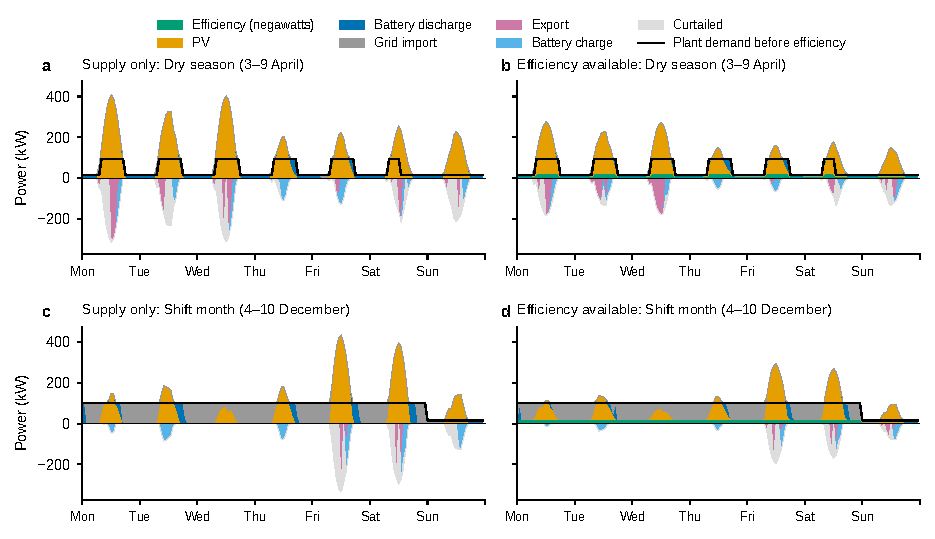
\includegraphics[width=\linewidth]{figures/fig10_urbs_dispatch.pdf}
\end{adjustwidth}
\caption{Hourly operation of the cost-optimal systems for a 20\% emission cap: (a,b) supply only; (c,d) efficiency available.}
\label{fig:urbsdispatch}
\end{figure}

\subsubsection{Battery cost}
Table~\ref{tab:urbsbat} repeats the optimisation with lower battery costs. Without an emission cap, batteries do not enter the optimum even at a quarter of the central cost, because under annual net metering the grid acts as a free and lossless store. Under a 20\% cap, halving the battery cost changes the optimal storage to \nUBatTwentyHalfE~kWh with efficiency and \nUBatTwentyHalfS~kWh without it, and at a quarter of the cost to \nUBatTwentyQuarterE\ and \nUBatTwentyQuarterS~kWh. Even then, efficiency lowers the annualised cost by \nUCostTwentyQuarterSave\%. Cheaper storage therefore does not displace efficiency; efficiency reduces both the storage required and the cost of every step along the frontier.

\begin{table}[H]
\caption{Effect of battery cost on the urbs optimum under net metering (battery in usable kWh).}
\label{tab:urbsbat}
\footnotesize
\resizebox{\linewidth}{!}{%
\begin{tabular}{lrrrrrrrrrrrr}
\toprule
 & \multicolumn{6}{c}{No emission cap} & \multicolumn{6}{c}{CO$_2$ cap 20\% of baseline} \\
\cmidrule(lr){2-7}\cmidrule(lr){8-13}
 & \multicolumn{3}{c}{Supply only} & \multicolumn{3}{c}{Efficiency available} & \multicolumn{3}{c}{Supply only} & \multicolumn{3}{c}{Efficiency available} \\
Battery cost & kWh & kWp & kMXN & kWh & kWp & kMXN & kWh & kWp & kMXN & kWh & kWp & kMXN \\
\midrule
100\% & 0 & 303 & 412 & 0 & 269 & 391 & 317 & 452 & 1{,}083 & 163 & 285 & 709 \\
75\% & 0 & 303 & 412 & 0 & 269 & 391 & 341 & 428 & 980 & 172 & 276 & 657 \\
50\% & 0 & 303 & 412 & 0 & 269 & 391 & 366 & 409 & 871 & 189 & 264 & 601 \\
25\% & 0 & 303 & 412 & 0 & 269 & 391 & 432 & 375 & 747 & 211 & 252 & 539 \\
\bottomrule
\end{tabular}}
\end{table}


\section{Discussion}
\label{sec:discussion}

\subsection{What efficiency first means at plant scale}
The results do not support a simple ``efficiency instead of solar'' narrative. Rooftop PV is a profitable investment for this plant, and the largest NPV is obtained by doing both. What EE1st changes is the order and size of the supply investment. Treating demand-side measures as a resource that competes with PV, as the principle requires~\cite{mandel2022,ec2021ee1st}, reveals that efficiency delivers the first \nEESavedPct\% of the reduction in grid purchases at low cost. It also shrinks the PV array needed for any higher target, by \nPVDiffFour~kWp in this case. That frees capital, roof area and grid-connection capacity for later steps such as heat electrification. The same logic underpins system-level EE1st analyses~\cite{mandel2023,pato2022}. Here it appears in the investment decision of a single SME.

The low cost of the operational measure (E4) deserves emphasis. Its value rests on the large production-independent load revealed by a simple baseline regression. Such loads are common in discrete manufacturing~\cite{kara2011,mouzon2007} but invisible in averaged indicators such as kWh per pair. Capturing these savings requires routines, sub-metering and accountability rather than capital, which is why energy management practices and ISO~50001 matter for SMEs~\cite{thollander2025,mckane2017}. Efficiency measures can also bring non-energy benefits, such as lower noise from compressed-air systems~\cite{nehler2018}. Insulating heated equipment would reduce heat gains in a plant where workers reported high indoor temperatures. These benefits are not monetised here, so the estimates for efficiency are conservative~\cite{worrell2003,nehler2016}.

\subsection{Tariff design as a hidden driver}
The tariff analysis explains why both efficiency and PV look attractive. Under GDMTO the capacity charge, and in practice also the distribution charge, is computed from monthly energy divided by a fixed load factor~\cite{dof2025tariffs}. This turns demand charges into a volumetric charge and raises the value of an avoided kWh to \nTMarg~\MXN, \nTEnergyShare\% of which is the energy charge. For efficiency the design is benign, since saved kWh are worth the same whatever their timing. For PV it creates a regulatory dependency, because most of its value rests on net-metered generation reducing the billed demand. The stress case shows that a change in that rule would remove most of the PV's NPV while leaving efficiency untouched. An EE1st appraisal that uses only an average price would miss this asymmetry. The finding echoes the importance of incentive design stressed by Pato et al.~\cite{pato2022}, seen here from the customer's side of the meter. The bills also suggest that the plant's measured peaks exceed the 100~kW GDMTO limit. Under the time-of-use GDMTH tariff, capacity is billed on demand coincident with the evening peak period and energy is priced by period~\cite{dof2025tariffs}. Base-load reductions that persist into the peak period would then gain value, whereas daytime PV output would contribute little to peak-period demand. Reclassification would therefore be likely to widen the advantage of efficiency first, although this was not simulated.

\subsection{Energy security and the phase-out of fossil fuels}
Because two-thirds of Mexican grid electricity is gas-fired and roughly three-quarters of the gas is imported~\cite{sener2025plan,eia2025mexico}, every kWh saved or self-generated by an SME reduces the country's exposure to an external fuel supply. At the plant level, efficiency and PV reduce exposure to an energy-charge shock by similar amounts for the same reduction in grid purchases. Efficiency, however, does so without regulatory risk, without roof constraints and while lowering demand. For the phase-out of fossil fuels, the thermal analysis adds a nuance. Electrification of heat is economically compelling against LPG but not yet against pipeline gas. Efficiency first makes room for electrification by freeing grid capacity and lowering the plant's peak. The official emission factor has not declined in recent years. Behind-the-meter efficiency is therefore the decarbonisation lever least dependent on progress in the grid.

\subsection{Can the plant reach net zero?}
For electricity, yes, on an annual basis and at a profit under current rules: an efficiency-first plant with about \nKWpNZE~kWp of rooftop PV generates as much as it consumes. Two qualifications matter for how such a claim is made. First, annual netting is not equivalent to zero emissions in a location-based inventory: about \nCOGrossNZE~tCO$_2$ per year of grid imports remain, mostly at night and in the winter shift months, even though exports displace a similar amount of grid generation during the day. Second, physical self-sufficiency above about \nFirstBattery\% requires batteries whose cost is not recovered under net metering, net billing or energy-based demand charges. A net-zero claim for this plant should therefore be framed as annual net-zero electricity, with gross imports and location-based emissions reported alongside~\cite{iso50001}. Storage becomes attractive only if battery costs fall by at least three-quarters, if compensation rules penalise exports more than in the cases tested, or if the firm values resilience to outages explicitly. Efficiency first reduces the cost of every one of these steps, chiefly by shrinking the consumption that PV and storage must cover, and with it the array and the roof. Full net zero also requires the thermal fuels discussed in Section~\ref{sec:thermal} to be electrified, which the electricity headroom created by efficiency makes easier.

\subsection{What formal optimisation adds}
The urbs results support the sequencing rule and refine it. In the linear programme, efficiency is not placed first by assumption: it competes with PV, storage and grid purchases in every hour, and the optimiser chooses it first. Its order of adoption reproduces the conservation supply curve. Base-load control and insulation are adopted in every scenario, and the servo motors and the compressed-air package are adopted as soon as the value of PV output falls below the tariff. Under generous annual net metering, PV output is worth the full tariff, so the two measures whose CCE is slightly above the PV LCOE are not selected even though each is profitable on its own (Table~\ref{tab:measures}); the ranking between PV and these two measures is also uncertain in the Monte Carlo analysis. When roof area, export compensation or an emission cap binds, the full efficiency bundle enters first and lowers the cost of every subsequent step. These conditions characterise the deeper stages of decarbonisation, and the steps include the storage that physical self-sufficiency requires. Efficiency first is therefore an emergent property of least-cost design under constraints, not only a normative principle.

The optimisation also shows where the heuristic methods are sufficient and where they are not. The supply-only net-zero design of the linear programme coincides with that of the hourly design search, which the toolkit implements and which handles the monthly credit bank and the three billing rules explicitly. For shallow targets, sizing PV after efficiency and following the merit order therefore capture the main trade-offs. For deep targets, the joint optimisation is needed. It co-ordinates measures, PV, storage and curtailment hour by hour, and it reveals that the cost of the last tonnes of CO$_2$ is dominated by storage, which efficiency reduces but cannot remove. For SMEs facing emission targets from customers or lenders, this suggests a two-stage planning process. Simple tools can screen measures and size PV; an energy-system model such as urbs can then be used once storage or emission caps enter the decision.

\subsection{Implications for practice and policy}
For the plant, the results suggest a staged plan: (i) implement base-load control, PF correction and compressed-air maintenance immediately, as they are low-cost and verifiable; (ii) retrofit sewing motors and insulate heated equipment; (iii) size PV only after the savings have been measured; (iv) investigate thermal fuel use and heat recovery. The M\&V plan prepared during the audit already specifies IPMVP options for each measure~\cite{evo2022ipmvp} and is summarised in Appendix~\ref{app:mv}. For policy, three implications follow. First, distributed-generation programmes and green-credit lines aimed at SMEs could require an efficiency screening, such as a simple baseline regression and an audit, before PV sizing, in the spirit of the EU's EE1st guidance~\cite{ec2024ee1st}. Second, tariff reforms that move GDMTO demand charges towards measured peaks would strengthen incentives for demand management but erode the value of PV. They should therefore be signalled in advance. Third, the large share of production-independent load points to the value of energy-management networks and capacity building for SMEs~\cite{jalo2021,johansson2019,herce2024}. University research projects in which students apply energy-systems modelling to real decarbonisation problems are one route to building that capacity~\cite{garciakerdan2026educon}; the open framework and toolkit presented here are designed to be used in such projects.

\subsection{Transferability to other SMEs}
The analysis rests on data that most SMEs already hold or can obtain in a walk-through audit (Table~\ref{tab:datatiers}). Twelve months of bills and an end-use estimate are enough to rank measures against PV, to compare the supply-only and efficiency-first pathways and to compute the security indicators. A production series adds the baseline regression that identified the base load, the cheapest resource in this case. Hourly weather adds the net-zero analysis, and interval metering would replace the synthetic load profile, the weakest element of that analysis. The toolkit lists each input with its data status and its rank correlation with the NPV advantage of the efficiency-first portfolio across the Monte Carlo draws, so that a firm can see where the next measurement is worth making. Three results are likely to transfer: base-load control is cheap wherever production-independent load is large; efficiency first shrinks the PV array whenever the PV surplus is not remunerated; and storage is hard to justify under net metering. Others depend on the tariff. In particular, the regulatory risk to PV found here arises from Q-based demand charges; under a measured-peak tariff the toolkit assumes, conservatively, that PV earns no demand credit, whereas efficiency lowers the peak in proportion to its effect on average power, so efficiency would gain relative value.

\begin{table}[H]
\centering
\caption{Data tiers for applying the method to other SMEs.}
\label{tab:datatiers}
\footnotesize
\begin{tabular}{p{0.30\linewidth}p{0.62\linewidth}}
\toprule
Data & Analyses enabled \\
\midrule
12 monthly bills, tariff, end-use estimate, monthly climate & Tariff check, measure CCE and NPV, merit order, portfolios P1--P4, pathways, CO$_2$ and security indicators, Monte Carlo \\
+ monthly production & ISO~50006 baseline and base-load share \\
+ hourly weather year & Hourly PV, battery dispatch, net-zero and self-sufficiency frontier under three compensation regimes \\
+ interval metering & Measured always-on load in place of the assumed value (load shapes and time-of-use tariffs are not yet implemented) \\
+ fuel records & Scaling the per-GJ heat-electrification results to the plant \\
\bottomrule
\end{tabular}
\end{table}

\subsection{Limitations}
This is an ex-ante evaluation study, and its limits should be read alongside its findings.
\begin{itemize}
\item \emph{Data transcription.} Billing data were transcribed from utility bills rather than obtained from interval metering.
\item \emph{End-use split.} The split is an audit estimate for one month and is assumed constant across months.
\item \emph{Measure savings and costs.} Savings of E1--E4 and the costs of E2--E4 come from literature and market ranges rather than plant-specific measurements and quotations. The Monte Carlo analysis shows that the conclusions hold across these ranges, but the absolute savings must be verified through the M\&V plan.
\item \emph{PV and load models.} The main PV model is monthly. The net-zero analysis uses hourly PV for one weather year rescaled to climatology and a synthetic hourly load built from an assumed always-on load and scheduled operating hours; shading and actual load shapes are not resolved, and inverter clipping is represented only in the EnergyPlus runs. Both models convert the NASA POWER hourly time stamps (UTC$-7$ at this longitude) to local clock time; the EnergyPlus weather file assumes constant relative humidity (60\%) and wind speed (2~m~s$^{-1}$), which affect module temperature only slightly. Storage sizing in particular should be confirmed with interval data.
\item \emph{Demand ceiling.} Measured maximum demand is only implied by the load factors printed on the bills. The model assumes that the energy-based demand term remains binding, which is consistent with the billed demand.
\item \emph{Tariff migration.} Migration to GDMTH, which would apply time-of-use energy prices and capacity charges on peak-period demand, is discussed but not simulated because no interval data were available; the bills identify the plant as a GDMTO customer, which is the tariff modelled.
\item \emph{Thermal fuel use.} Because fuel consumption was not metered, the fuel-substitution analysis is parametric.
\item \emph{Energy-security indicators.} Imported gas embodied in grid electricity is estimated with average shares and an assumed heat rate rather than with marginal dispatch.
\item \emph{Linear programme.} The urbs model optimises one representative year with perfect foresight, values grid electricity at a constant marginal price, represents net metering as annual netting without the 12-month expiry of credits, omits PV degradation and battery ageing and allows partial adoption of measures. It is used to test the design logic and to trace the decarbonisation frontier rather than to size equipment exactly.
\end{itemize}
None of these simplifications favours efficiency systematically. Several are conservative, notably the exclusion of non-energy benefits and the zero value assigned to PV surplus.

%% ===================================================================
\section{Conclusions}
\label{sec:conclusions}

This study applied the energy efficiency first principle to the investment choices of a Mexican footwear SME, comparing demand-side measures with rooftop PV and heat electrification on common indicators of energy, emissions, cost and security.

The main conclusions are:
\begin{itemize}
\item \emph{Validated tariff model.} A model built from official GDMTO charges reproduces the plant's bills with a mean absolute error of \nTVMape\%. It shows that demand charges are effectively volumetric, so each avoided kWh is worth \nTMarg~\MXN.
\item \emph{Cost of demand-side measures.} Base-load control, insulation of heated equipment, servo motors and a compressed-air package together save \nEESavedPct\% of grid electricity. Their central costs of \nCCEBase--\nCCECA~\MXN~kWh$^{-1}$ are below even the energy charge alone, and their paybacks are at most \nPBMaxEE\ years.
\item \emph{Sequencing and PV sizing.} PV is profitable, but sequencing matters. Implementing efficiency first achieves the same \nGridTwo\% reduction in grid purchases with \nPVSaveFour\% less PV capacity, \nCapexSaveFour\% less capital and a higher NPV in \nProbFourTwo\% of uncertainty draws.
\item \emph{Security and resilience.} Efficiency lowers the plant's peak, preserves its value if distributed-generation compensation changes and reduces exposure to imported gas and to energy-price shocks.
\item \emph{Heat electrification.} Heat pumps outcompete LPG boilers above a COP of \nCOPBELPG, but not yet pipeline gas at current wholesale prices.
\item \emph{Net zero.} Annual net-zero electricity is achievable and profitable with \nKWpNZE--\nEPKWpNZE~kWp of PV after efficiency (Python and EnergyPlus sizing; \nNZKWpSave--\nEPKWpSave~kWp less than without it). Hourly self-sufficiency of 80\% needs \nBatSSE~kWh of storage and 90\% turns the NPV negative; under current rules storage is a resilience investment, not a cost saving.
\item \emph{Joint optimisation.} In an urbs linear programme that co-optimises the measures, PV, storage and hourly operation, efficiency is adopted before PV and storage. Under emission caps of 35--10\% of the baseline it lowers the annualised cost by \nUCapSaveMin--\nUCapSaveMax\% and delays and shrinks the battery, which dominates the cost of deep decarbonisation.
\end{itemize}

For SMEs in emerging economies, EE1st is best understood as a sequencing rule: measure, cut the waste, then size the supply. The open \texttt{ee1st} toolkit released with this paper allows other plants to repeat the assessment from twelve monthly bills and an end-use estimate, adding detail as production, weather or interval data become available. Future work should verify the savings ex post, add interval data to resolve hourly PV self-consumption and peak demand, and quantify thermal fuel use so that the phase-out of fossil fuels on site can be assessed directly.



\vspace{6pt}

\authorcontributions{Conceptualization, I.G.K.; methodology, I.A.G. and I.G.K.; software, I.G.K.; validation, S.A.R.-M. and I.G.K.; formal analysis, Y.A.A., F.A.S. and I.G.K.; investigation, Y.A.A., I.A.G. and F.A.S.; data curation, Y.A.A. and I.A.G.; writing---original draft preparation, I.G.K.; writing---review and editing, Y.A.A., I.A.G., F.A.S., S.A.R.-M. and I.G.K.; visualization, S.A.R.-M. and I.G.K.; supervision, I.G.K. All authors have read and agreed to the published version of the manuscript.}

\funding{This research received no external funding.}

\institutionalreview{Not applicable.}

\informedconsent{Not applicable.}

\dataavailability{The plant's billing, production and audit records are confidential and cannot be shared, because the company has not authorised their release; summary statistics are given in Table~\ref{tab:billing}. The model code, the public input data (tariffs, emission factors, fuel prices and climate), all derived results and the scripts that produce the tables and figures are openly available on Zenodo at \url{https://doi.org/10.5281/zenodo.23419738} (MIT licence for code; CC~BY~4.0 for data and results). The same deposit contains the generalised toolkit \texttt{ee1st} in its \texttt{ee1st/} folder.}

\acknowledgments{The authors thank the plant's maintenance manager and site staff for access to the facility and its records. During the preparation of this manuscript, the authors used Claude 5.5 (Anthropic) to a minimal extent, for language editing and checking of code. The authors have reviewed and edited the output and take full responsibility for the content of this publication.}

\conflictsofinterest{I.G.K. is the Guest Editor of the Special Issue ``Advanced Modelling, Optimisation and AI for Sustainable Energy Systems'' of \emph{Processes} and acts as an Academic Editor for \emph{Processes}. In accordance with MDPI's Special Issue policy, this manuscript is to be handled by an independent Academic Editor, and I.G.K. will have no access to its peer-review process other than as an author. The other authors declare no conflicts of interest.}

\abbreviations{Abbreviations}{
The following abbreviations are used in this manuscript:\\

\noindent
\begin{tabular}{@{}ll}
CCE & Cost of conserved energy\\
CFE & Comisión Federal de Electricidad (Federal Electricity Commission)\\
COP & Coefficient of performance\\
CRE & Comisión Reguladora de Energía (Energy Regulatory Commission)\\
CV-RMSE & Coefficient of variation of the root-mean-square error\\
DG & Distributed generation\\
EE1st & Energy efficiency first\\
EnB & Energy baseline\\
EPW & EnergyPlus weather file\\
GDMTH & Hourly large demand, medium-voltage tariff\\
GDMTO & Ordinary large demand, medium-voltage tariff\\
IPMVP & International Performance Measurement and Verification Protocol\\
LCOE & Levelised cost of electricity\\
LPG & Liquefied petroleum gas\\
M\&V & Measurement and verification\\
MXN & Mexican peso\\
NPV & Net present value\\
PF & Power factor\\
PV & Photovoltaics\\
SME & Small and medium-sized enterprise\\
VAT & Value-added tax
\end{tabular}
}

%=================================================================

\appendixtitles{yes}
\appendixstart
\appendix


\section{Billing, production and tariff data}
\label{app:data}
The monthly records were transcribed from utility bills and plant production records; they are confidential and only their summary is reproduced (Table~\ref{tab:billing}). Table~\ref{tab:tariffs} lists the official tariff charges for Pachuca de Soto.
\begin{table}[H]
\centering
\caption{Billing and production records, January 2024--April 2026 (summary only; monthly data confidential).}
\label{tab:billing}
\footnotesize
\begin{tabular}{lrrrr}
\toprule
Variable & Months & Minimum & Mean & Maximum \\
\midrule
Electricity (kWh per month) & 28 & 19{,}040 & 35{,}523 & 64{,}160 \\
Billed demand (kW) & 28 & 46 & 89 & 157 \\
Power factor (\%) & 28 & 84.4 & 87.1 & 90.6 \\
Average price (MXN kWh$^{-1}$, pre-VAT) & 28 & 2.770 & 3.005 & 3.153 \\
Production (pairs per month) & 25 & 3{,}473 & 13{,}692 & 29{,}460 \\
\bottomrule
\end{tabular}
\end{table}

\begin{table}[H]
\centering
\caption{Official GDMTO charges, Centro Oriente division, pre-VAT \citep{cfe2026gdmto}.}
\label{tab:tariffs}
\footnotesize
\resizebox{\linewidth}{!}{%
\begin{tabular}{lrrrr}
\toprule
Month & Fixed (MXN month$^{-1}$) & Energy (MXN kWh$^{-1}$) & Distribution (MXN kW$^{-1}$) & Capacity (MXN kW$^{-1}$) \\
\midrule
2024-01 & 360.01 & 1.544 & 155.26 & 342.36 \\
2024-02 & 360.01 & 1.552 & 155.26 & 344.34 \\
2024-03 & 360.01 & 1.569 & 155.26 & 348.69 \\
2024-04 & 360.01 & 1.569 & 155.26 & 348.70 \\
2024-05 & 360.01 & 1.569 & 155.26 & 348.70 \\
2024-06 & 360.01 & 1.569 & 155.26 & 348.70 \\
2024-07 & 360.01 & 1.608 & 155.26 & 358.56 \\
2024-08 & 360.01 & 1.621 & 155.26 & 361.67 \\
2024-09 & 360.01 & 1.621 & 155.26 & 361.69 \\
2024-10 & 360.01 & 1.621 & 155.26 & 361.70 \\
2024-11 & 360.01 & 1.621 & 155.26 & 361.69 \\
2024-12 & 360.01 & 1.597 & 155.26 & 355.67 \\
2025-01 & 308.10 & 1.617 & 155.81 & 359.79 \\
2025-02 & 308.10 & 1.620 & 155.81 & 360.36 \\
2025-03 & 308.10 & 1.620 & 155.81 & 360.51 \\
2025-04 & 308.10 & 1.620 & 155.81 & 360.51 \\
2025-05 & 308.10 & 1.620 & 155.81 & 360.51 \\
2025-06 & 308.10 & 1.654 & 155.81 & 369.07 \\
2025-07 & 308.10 & 1.676 & 155.81 & 374.61 \\
2025-08 & 308.10 & 1.678 & 155.81 & 375.13 \\
2025-09 & 308.10 & 1.668 & 155.81 & 371.70 \\
2025-10 & 308.10 & 1.668 & 155.81 & 371.70 \\
2025-11 & 308.10 & 1.624 & 155.81 & 360.54 \\
2025-12 & 308.10 & 1.553 & 155.81 & 342.52 \\
2026-01 & 335.36 & 1.519 & 149.44 & 334.81 \\
2026-02 & 335.36 & 1.520 & 149.44 & 335.00 \\
2026-03 & 335.36 & 1.521 & 149.44 & 335.20 \\
2026-04 & 335.36 & 1.521 & 149.44 & 335.19 \\
2026-05 & 335.36 & 1.508 & 149.44 & 331.84 \\
2026-06 & 335.36 & 1.495 & 149.44 & 328.54 \\
2026-07 & 335.36 & 1.469 & 149.44 & 321.97 \\
2026-08 & 335.36 & 1.469 & 149.44 & 321.98 \\
2026-09 & 335.36 & 1.469 & 149.44 & 321.98 \\
2026-10 & 335.36 & 1.469 & 149.44 & 321.98 \\
\bottomrule
\end{tabular}}
\end{table}


\section{Model parameters}
\label{app:params}
Table~\ref{tab:parameters} lists the model parameters. Ranges define triangular distributions whose mode is the central value. Status codes: M measured, O official, O* derived from official data, L literature, Q quotation in the audit report, D design, A assumption, R regulatory scenario. The last nine parameters belong to the hourly net-zero module (Section~\ref{sec:nzmethod}) and are varied in scenario analysis only.
{\footnotesize
\begin{longtable}{p{3.4cm}rlcp{4.0cm}}
\caption{Model parameters, ranges and status.}\label{tab:parameters}\\
\toprule
Parameter & Central & Range & Status & Source / note \\
\midrule
\endfirsthead
\toprule
Parameter & Central & Range & Status & Source / note \\
\midrule
\endhead
\texttt{discount\_\allowbreak{}rate} & 0.1 & 0.06--0.14 & A & student report; sensitivity \\
\texttt{horizon\_\allowbreak{}yr} & 20 & fixed & A & student report \\
\texttt{tariff\_\allowbreak{}real\_\allowbreak{}escalation} & 0 & -0.01--0.02 & A & constant real tariffs \\
\texttt{ef\_\allowbreak{}grid\_\allowbreak{}t\_\allowbreak{}per\_\allowbreak{}MWh} & 0.444 & fixed & O & \cite{semarnat2025fesen} \\
\texttt{gas\_\allowbreak{}share\_\allowbreak{}generation} & 0.638 & 0.6--0.68 & O & \cite{sener2025plan} Tabla 2.2 \\
\texttt{ccgt\_\allowbreak{}heat\_\allowbreak{}rate\_\allowbreak{}GJ\_\allowbreak{}per\_\allowbreak{}MWh} & 7.2 & 6.5--8.5 & A & typical CCGT 42-55\% LHV \\
\texttt{gas\_\allowbreak{}import\_\allowbreak{}share} & 0.74 & 0.7--0.78 & O* & \cite{eia2025mexico} 6.4/8.6 Bcf/d \\
\texttt{ca\_\allowbreak{}saving\_\allowbreak{}frac} & 0.2 & 0.1--0.3 & L & \cite{doe2016compressed} leaks 20-30\% -> <10\%; 1\%/2 psi \\
\texttt{ca\_\allowbreak{}capex} & 50000 & 35000--80000 & Q & student estimate \\
\texttt{ca\_\allowbreak{}om} & 8000 & 5000--12000 & A & annual ultrasonic leak survey \\
\texttt{ca\_\allowbreak{}life} & 10 & fixed & A &  \\
\texttt{sew\_\allowbreak{}motor\_\allowbreak{}share} & 0.7 & 0.5--0.85 & A & share of stitching-area energy in clutch motors \\
\texttt{sew\_\allowbreak{}saving\_\allowbreak{}frac} & 0.65 & 0.5--0.75 & L & \cite{nemesa2023} \\
\texttt{sew\_\allowbreak{}motor\_\allowbreak{}kW} & 0.35 & 0.25--0.45 & L & clutch motor running power \\
\texttt{sew\_\allowbreak{}cost\_\allowbreak{}per\_\allowbreak{}unit} & 3800 & 2800--5500 & A & installed servo motor, market \\
\texttt{sew\_\allowbreak{}life} & 10 & fixed & A &  \\
\texttt{heat\_\allowbreak{}share} & 0.65 & 0.5--0.8 & A & heater share of vulcanising+injection energy \\
\texttt{heat\_\allowbreak{}saving\_\allowbreak{}frac} & 0.2 & 0.1--0.3 & L & \cite{kent2018}; grey literature 15-30\% \\
\texttt{heat\_\allowbreak{}capex} & 100000 & 60000--150000 & A & jackets + controls \\
\texttt{heat\_\allowbreak{}life} & 8 & fixed & A &  \\
\texttt{base\_\allowbreak{}saving\_\allowbreak{}frac} & 0.1 & 0.05--0.2 & L & \cite{mouzon2007}; \cite{kara2011} \\
\texttt{base\_\allowbreak{}capex} & 40000 & 20000--70000 & A & timers, contactors, sub-meters \\
\texttt{base\_\allowbreak{}life} & 10 & fixed & A &  \\
\texttt{pfc\_\allowbreak{}kvar} & 50 & fixed & Q & student design \\
\texttt{pfc\_\allowbreak{}pf\_\allowbreak{}after} & 0.97 & 0.95--0.99 & A & automatic bank \\
\texttt{pfc\_\allowbreak{}capex} & 85000 & 70000--110000 & Q & student estimate \\
\texttt{pfc\_\allowbreak{}life} & 15 & fixed & A &  \\
\texttt{pv\_\allowbreak{}kWp} & 163.8 & fixed & D & 252 x 650 W modules (student design) \\
\texttt{pv\_\allowbreak{}cost\_\allowbreak{}per\_\allowbreak{}W} & 11 & 9--14 & Q & student quote 1.8 MMXN / 163.8 kWp \\
\texttt{pv\_\allowbreak{}PR} & 0.8 & 0.75--0.85 & L & \cite{reich2012} \\
\texttt{pv\_\allowbreak{}tilt\_\allowbreak{}deg} & 20 & fixed & D & latitude tilt \\
\texttt{pv\_\allowbreak{}albedo} & 0.2 & fixed & A &  \\
\texttt{pv\_\allowbreak{}degradation} & 0.005 & 0.003--0.008 & L & typical crystalline Si \\
\texttt{pv\_\allowbreak{}om\_\allowbreak{}frac} & 0.01 & 0.005--0.015 & A & of capex per year \\
\texttt{pv\_\allowbreak{}inverter\_\allowbreak{}repl\_\allowbreak{}frac} & 0.1 & 0.08--0.15 & A & of capex at year 12 \\
\texttt{pv\_\allowbreak{}life} & 25 & fixed & L &  \\
\texttt{pv\_\allowbreak{}m2\_\allowbreak{}per\_\allowbreak{}kWp} & 5.5 & 5--6.5 & A & 650 W module 3.1 m2 incl. spacing \\
\texttt{pv\_\allowbreak{}demand\_\allowbreak{}credit} & 1 & 0--1 & R & net metering reduces Q-based billed demand \\
\texttt{lpg\_\allowbreak{}price\_\allowbreak{}MXN\_\allowbreak{}per\_\allowbreak{}kg\_\allowbreak{}incl\_\allowbreak{}vat} & 19.76 & fixed & O & CNE max price, PROFECO 11-17 Oct 2026 \\
\texttt{lpg\_\allowbreak{}LHV\_\allowbreak{}MJ\_\allowbreak{}per\_\allowbreak{}kg} & 47.3 & fixed & L & IPCC 2006 Vol.2 Table 1.2 NCV \\
\texttt{lpg\_\allowbreak{}EF\_\allowbreak{}kg\_\allowbreak{}per\_\allowbreak{}GJ} & 63.1 & fixed & L & IPCC 2006 Vol.2 Table 2.2 \\
\texttt{ng\_\allowbreak{}EF\_\allowbreak{}kg\_\allowbreak{}per\_\allowbreak{}GJ} & 56.1 & fixed & L & IPCC 2006 Vol.2 Table 2.2 \\
\texttt{ng\_\allowbreak{}enduser\_\allowbreak{}markup} & 2 & 1.5--3 & A & transport+distribution over IPGN \\
\texttt{boiler\_\allowbreak{}eff} & 0.85 & 0.8--0.9 & A &  \\
\texttt{hp\_\allowbreak{}cop} & 3 & 2.5--4 & L & \cite{arpagaus2018}; \cite{schlosser2020} (<100 C) \\
\texttt{ca\_\allowbreak{}heat\_\allowbreak{}recovery\_\allowbreak{}frac} & 0.7 & 0.5--0.8 & L & \cite{doe2016compressed} >80\% available \\
\texttt{night\_\allowbreak{}load\_\allowbreak{}kW} & 15 & 8--25 & A & always-on load outside shifts; needs interval data \\
\texttt{bat\_\allowbreak{}cost\_\allowbreak{}per\_\allowbreak{}kWh} & 8500 & fixed & A & installed C\&I LFP; NREL ATB 2024 (\citealp{nrel2024atb}) pack 199 USD/kWh + inverter/BOS \\
\texttt{bat\_\allowbreak{}rte} & 0.85 & fixed & L & NREL ATB 2024 (\citealp{nrel2024atb}) commercial battery \\
\texttt{bat\_\allowbreak{}dod} & 0.9 & fixed & A & usable fraction of nameplate \\
\texttt{bat\_\allowbreak{}c\_\allowbreak{}rate} & 0.5 & fixed & A & kW per kWh \\
\texttt{bat\_\allowbreak{}om\_\allowbreak{}frac} & 0.025 & fixed & L & NREL ATB 2024 (\citealp{nrel2024atb}): 2.5\% of capex per year \\
\texttt{bat\_\allowbreak{}life} & 15 & fixed & L & NREL ATB 2024 (\citealp{nrel2024atb}) \\
\texttt{expired\_\allowbreak{}credit\_\allowbreak{}value} & 0 & 0--1 & A & MXN/kWh paid for credits older than 12 months (PML); 0 = conservative \\
\texttt{net\_\allowbreak{}billing\_\allowbreak{}export\_\allowbreak{}value} & 1 & 0.6--1.5 & A & MXN/kWh export value in a net-billing stress case \\
\bottomrule
\end{longtable}}


\section{Photovoltaic resource and yield}
\label{app:pv}
Monthly mean daily plane-of-array irradiation $\bar H_T$ was computed from NASA POWER monthly mean global ($\bar H$) and diffuse ($\bar H_d$) horizontal irradiation~\cite{nasapower} as
\begin{equation}
\bar H_T = \bar H\left[\left(1-\frac{\bar H_d}{\bar H}\right)\bar R_b + \frac{\bar H_d}{\bar H}\,\frac{1+\cos\beta}{2} + \rho_g\,\frac{1-\cos\beta}{2}\right],
\end{equation}
with the monthly beam tilt factor $\bar R_b$ of Klein~\cite{klein1977} for a south-facing surface evaluated on each month's recommended day, tilt $\beta = 20^\circ$ and ground reflectance $\rho_g=0.2$. Annual mean horizontal irradiation is \nGHI~kWh~m$^{-2}$~d$^{-1}$, compared with the 4.8 peak-sun hours used in the audit report, and plane-of-array irradiation is \nPOA~kWh~m$^{-2}$~d$^{-1}$. With a performance ratio of 0.80 the specific yield is \nSpecYield~kWh~kWp$^{-1}$~yr$^{-1}$. The audit report sized the array at \nStuKWp~kWp to cover 80\% of a 28,400~kWh month with 4.8 peak-sun hours and no performance ratio, and proposed 252 modules (\nStuKWpMod~kWp). This study adopts the module-based capacity.

\section{Sensitivity analysis}
\label{app:sens}
Table~\ref{tab:sensitivity} gives the 20-year NPV of each portfolio with each parameter at its low and high bound and all others at their central values, ranked by the swing of P4.
\begin{table}[H]
\centering
\caption{One-way sensitivity of 20-year NPV (MMXN).}
\label{tab:sensitivity}
\footnotesize
\resizebox{\linewidth}{!}{%
\begin{tabular}{lrrrrrr}
\toprule
 & \multicolumn{2}{c}{P1 Efficiency} & \multicolumn{2}{c}{P2 PV only} & \multicolumn{2}{c}{P4 Efficiency first} \\
Parameter & low & high & low & high & low & high \\
\midrule
\texttt{discount\_rate} & 2.64 & 1.33 & 5.42 & 2.39 & 5.64 & 2.64 \\
\texttt{tariff\_real\_escalation} & 1.68 & 2.22 & 3.23 & 4.34 & 3.45 & 4.62 \\
\texttt{base\_saving\_frac} & 1.56 & 2.40 & 3.57 & 3.57 & 3.53 & 4.36 \\
\texttt{pv\_cost\_per\_W} & 1.84 & 1.84 & 3.92 & 3.03 & 4.01 & 3.50 \\
\texttt{heat\_saving\_frac} & 1.60 & 2.08 & 3.57 & 3.57 & 3.57 & 4.04 \\
\texttt{pv\_PR} & 1.84 & 1.84 & 3.22 & 3.91 & 3.61 & 4.00 \\
\texttt{sew\_saving\_frac} & 1.64 & 1.97 & 3.57 & 3.57 & 3.61 & 3.94 \\
\texttt{ca\_saving\_frac} & 1.68 & 2.00 & 3.57 & 3.57 & 3.65 & 3.96 \\
\texttt{sew\_motor\_share} & 1.69 & 1.95 & 3.57 & 3.57 & 3.66 & 3.92 \\
\texttt{sew\_cost\_per\_unit} & 1.93 & 1.69 & 3.57 & 3.57 & 3.89 & 3.66 \\
\texttt{heat\_share} & 1.73 & 1.95 & 3.57 & 3.57 & 3.70 & 3.91 \\
\texttt{sew\_motor\_kW} & 1.71 & 1.91 & 3.57 & 3.57 & 3.67 & 3.88 \\
\bottomrule
\end{tabular}}
\end{table}


\section{Measurement and verification plan}
\label{app:mv}
The audit team prepared an M\&V plan following IPMVP~\cite{evo2022ipmvp}. PV output is verified under Option~B through inverter and bidirectional-meter data with local irradiance. The capacitor bank is verified under Option~C through billed PF and surcharges, or Option~B where a network analyser is installed. Compressed air is verified under Option~B through dedicated metering of kWh, pressure and operating hours, with specific consumption (kWh per m$^3$ of air) as the indicator where flow can be measured. Servo motors and insulation can be verified under Option~A with spot power measurements and logged hours. Base-load control is verified under Option~C through the production-normalised baseline of Section~\ref{sec:method}, complemented by night and weekend load readings. The whole facility is verified under Option~C with at least 12 months of post-implementation billing, adjusted for production and operating hours. Given the CV-RMSE of the baseline (\nCVExcl\%), savings below about 10\% of consumption cannot be detected reliably at whole-facility level. Sub-metering of the compressed-air room and of the vulcanising and stitching areas is therefore recommended as the first implementation step.



\begin{adjustwidth}{-\extralength}{0cm}
\reftitle{References}
\bibliography{references}
\PublishersNote{}
\end{adjustwidth}
\end{document}
